\documentclass[11pt]{article}
\usepackage[T1]{fontenc}
\usepackage[utf8]{inputenc}
\usepackage{lmodern}
\input{glyphtounicode.tex}
\input{glyphtounicode-cmex.tex}
\pdfglyphtounicode{mapsto}{007C}
\pdfglyphtounicode{vextendsingle}{23D0}
\pdfglyphtounicode{vextenddouble}{2016}
\pdfgentounicode=1
\usepackage[margin=1in]{geometry}
\usepackage{amsmath,amssymb,amsthm,mathtools}
\usepackage{microtype}
\usepackage{booktabs}
\usepackage{enumitem}
\usepackage{tikz}
\usetikzlibrary{arrows.meta,calc,positioning}
\usepackage{xcolor}
\definecolor{linkblue}{RGB}{24,64,111}
\usepackage[colorlinks=true,linkcolor=linkblue,citecolor=linkblue,urlcolor=linkblue,
  pdftitle={An exact Hausdorff gauge for SLE: a moment-integral and finite-batch construction},pdfauthor={OpenAI}]{hyperref}
\newcommand{\HH}{\mathbb H}
\newcommand{\DD}{\mathbb D}
\newcommand{\PP}{\mathbb P}
\newcommand{\EE}{\mathbb E}
\newcommand{\dd}{\mathop{}\!\mathrm{d}}
\newcommand{\ind}{\mathbf 1}
\newcommand{\SLE}{\mathrm{SLE}}
\newcommand{\Haus}{\mathcal H}
\newcommand{\supp}{\operatorname{supp}}
\newcommand{\diam}{\operatorname{diam}}
\newcommand{\dist}{\operatorname{dist}}
\newcommand{\Var}{\operatorname{Var}}
\newtheorem{theorem}{Theorem}[section]
\newtheorem{lemma}[theorem]{Lemma}
\newtheorem{proposition}[theorem]{Proposition}
\newtheorem{corollary}[theorem]{Corollary}
\theoremstyle{definition}
\newtheorem{definition}[theorem]{Definition}
\theoremstyle{remark}
\newtheorem{remark}[theorem]{Remark}
\numberwithin{equation}{section}
\setlist[enumerate]{itemsep=3pt,topsep=5pt}
\setlist[itemize]{itemsep=3pt,topsep=5pt}
\allowdisplaybreaks[2]


\title{An exact Hausdorff gauge for SLE\\[4pt]
\large A moment-integral and finite-batch construction}
\author{OpenAI}
\date{September 25, 2026}
\begin{document}
\maketitle
\begin{abstract}
For each \(0<\kappa<8\), we construct a deterministic Hausdorff gauge
that almost surely assigns positive finite measure to every nontrivial
compact positive-time segment of chordal Schramm--Loewner evolution.
This answers Schramm's Hausdorff-measure existence problem in this
parameter range. The entire trace has finite expected gauge measure
in each bounded box.
\end{abstract}
\section{Introduction}\label{sec:introduction}

A Hausdorff dimension identifies a critical power of distance, but that
power need not assign nonzero measure to a random curve. For chordal
Schramm--Loewner evolution $\SLE_\kappa$, $0<\kappa<8$, Beffara
\cite{Beffara2008} proved that the almost-sure dimension is
\[
 d=1+\frac\kappa8.
\]
Schramm asked whether the trace has a sigma-finite Hausdorff measure
and suggested $r^d\log\log(1/r)$ as a possible gauge
\cite[Problem~7.1 and the following paragraph]{Schramm2006}.
Rezaei subsequently proved that the critical power $r^d$ itself gives
zero Hausdorff measure \cite[Theorem~1.1]{Rezaei2018}.
The question therefore asks for a deterministic refinement of dimension
that measures the trace through arbitrary spatial covers.

We answer the existence question positively by constructing the scales
of the gauge from moments of a local trace mass. The gauge is explicit
in terms of deterministic integrals, although its asymptotics need not
have a regular form. The main mechanism uses finite moments of every
order in two ways: moderately large masses provide repeated opportunities
for an economical cover, while exceedances of a larger threshold have a
summable total cost. A sharp tail asymptotic is not needed.

\subsection{The result}

A \emph{Hausdorff gauge} is a continuous nondecreasing function
$h:[0,\infty)\to[0,\infty)$ with $h(0)=0$ and $h(r)>0$ for $r>0$.
We use diameters in the definition
\[
 \Haus^h(E)=\lim_{\delta\downarrow0}\Haus^h_\delta(E),\qquad
 \Haus^h_\delta(E)=\inf\left\{\sum_j h(\diam U_j):
 E\subset\bigcup_jU_j,\quad\diam U_j\le\delta\right\},
\]
where covers are countable and their sets may be arbitrary.

\begin{theorem}[An exact moment gauge]\label{thm:main}
Fix $0<\kappa<8$, and let $\gamma$ be chordal $\SLE_\kappa$ from
$0$ to $\infty$ in the upper half-plane $\HH$, parametrized by half-plane capacity $2t$.
There is a deterministic Hausdorff gauge $h_\kappa$, depending only on
$\kappa$, such that almost surely, simultaneously for every real
$0<s<t<\infty$,
\[
 0<\Haus^{h_\kappa}(\gamma([s,t]))<\infty.
\]
\end{theorem}

The gauge is the full infimum in \eqref{gauge:definition}, with
coefficients specified by the iterated integrals in \eqref{coef:formula}.
The exceptional event may depend on the fixed $\kappa$; the gauge
is independent of both the sample and the interval.
In particular, the trace outside its initial point has a nonzero
sigma-finite Hausdorff measure.

The upper argument measures the entire trace in a bounded region.
For $\Gamma=\gamma([0,\infty))$ and
$B_m=[-m,m]+i[0,m]$, Proposition~\ref{hd:upper} proves
\begin{equation}
 \EE\,\Haus^{h_\kappa}(\Gamma\cap B_m)<\infty
 \qquad(m\in\mathbb N).
 \label{intro:box-mean}
\end{equation}
Thus all these bounded-box measures are finite on one event, including
at real-boundary trace points. Positivity in Theorem~\ref{thm:main}
is asserted for the stated positive-time intervals.

\subsection{Multipoint estimates and one canonical mass}

The gauge construction needs a trace mass with moments of every order
and a way to compare its future in a small region with one fixed disk
model. We establish these inputs through a multipoint probability bound
and a conformally restarting mass. Both are also useful independently.
We first give a direct product-supermartingale proof of the fixed-order
estimate needed in an arbitrary physical domain.
For a conformal map $J:\HH\to D$, let $R_D(x)$ denote full conformal
radius: $R_D(x)=|F'(0)|$ when $F:\DD\to D$ is conformal,
$\DD$ is the unit disk, and $F(0)=x$.
Write $H_t$ for the surviving half-plane domain after the trace up to
time $t$, and $D_t=J(H_t)$. A point is \emph{alive} at $t$ when it
belongs to $D_t$; its evolving radius is $R_{D_t}(x)$.
Set $\alpha=2-d$ and $a=2/\kappa$.
For distinct interior points $x_1,\ldots,x_m$, choose caps satisfying
\[
 0<b_i\le R_D(x_i),\qquad b_i\le |x_i-x_j|\quad(j\ne i).
\]
Proposition~\ref{mp:estimate} proves that the probability that each point
reaches its own radius target $e_i>0$ while alive is at most
\begin{equation}
 C_{m,a}\prod_{i=1}^m\min\{1,(e_i/b_i)^\alpha\}.
 \label{intro:multipoint}
\end{equation}
The constant depends only on the fixed order and parameter. It is
uniform in the domain, the initial angles, and the order and times of
the hits. A completed point may be swallowed before another target is
reached. No sharp growth estimate in $m$ is claimed. Integrating the
collision singularities in this bound gives all the compact moments
used in the mass construction.

The second ingredient is a single adapted increasing measure process
$\mu_t$ on the open domain, starting at zero. In the half-plane,
Proposition~\ref{mass:construction} constructs it with nonatomic terminal
measure, local total-variation continuity, and increments carried by the
corresponding trace segments. Every nontrivial time interval has positive
increment mass by Proposition~\ref{mass:positive}.
To describe its conditional mean, let $g_S$ be the Loewner map of the
surviving half-plane domain $H_S$, with driving point $U_S$ in the
capacity normalization. For $x\in H_S$ put
$\theta_S(x)=\arg(g_S(x)-U_S)$ and
$G_S(x)=R_{H_S}(x)^{-\alpha}\sin^{8/\kappa-1}\theta_S(x)$;
put $G_S(x)=0$ outside $H_S$. Its remaining conditional mean is
\[
 \EE[\mu_\infty-\mu_S\mid\mathcal F_S]=G_S\,\dd A
\]
for every fixed stopping time $S$, including $S=\infty$ with
$G_\infty=0$. Here $\dd A$ is planar area. The equality holds as a
conditional measure kernel, so it includes nonnegative tests known
at $S$.

Conformal covariance weights the measure by $|J'|^d$.
At each fixed finite stopping time, Proposition~\ref{mass:restart}
identifies the actual future increment with the conformally transported
canonical mass of the fresh driver, simultaneously at every later time.
This permits comparison of the actual mass near a marked point with
one disk model after stopping at a prescribed conformal radius.
The lower bound also uses first-visit accounting: mass already
accumulated on the trace is not charged again at a later geometric return.

\subsection{Why the moments determine the gauge}

To bias the curve toward a marked interior point, stop when that point's
conformal radius reaches a prescribed smaller value and reweight the
stopped law by the ratio of its terminal and initial Green weights.
Paths that fail to reach the radius level receive weight zero.
Section~\ref{op:section} proves that the weight has mean one and that
these finite stopped laws are consistent as the radius decreases.
We call them the \emph{centered laws}.

Place the marked point at the origin of a unit disk and measure mass in
its radius-$1/4$ subdisk. The \emph{inner time} is the logarithmic radius
clock $\ell=(2a)^{-1}\log(R_0/R)$, where $R$ is the marked point's current
conformal radius. Let $L_\ell$ be the mass accumulated in that subdisk
by inner time $\ell$. Under the centered law, the marked point's angle
in the corresponding half-plane coordinates evolves as a diffusion
with invariant density proportional to
$\sin^{4a}\theta$. We average the initial angle against this distribution
and write
$\PP_{\mathrm{mix}}^*,\EE_{\mathrm{mix}}^*$ for this averaged centered
law and expectation. Then
\[
 L_\ell\uparrow L,\qquad 0<\EE_{\mathrm{mix}}^*L^n<\infty\quad(n\ge1).
\]
Section~\ref{coef:section} specifies these numbers by Wiener, angle and
area integrals, and then by product-normal coordinates and ordinary
differential equation limits. This deterministic infinite-limit
prescription fixes the normalization
of the moments without referring to an unspecified random measure.

For each order $n$, retain more than three quarters of its moment at a
finite level $\ell_n$. Repeat dyadic thresholds $A_k=2^k$ in a finite
batch with multiplicities $N_{nk}$ determined by the $n$th and
$(n+1)$st moments. Lemma~\ref{gauge:multiplicity} gives the complementary
bounds
\[
 \sum_kN_{nk}\PP_{\mathrm{mix}}^*\{L\ge16A_k\}
 \le\frac{4^{-n}}{1-2^{-n}},\qquad
 \sum_kN_{nk}\PP_{\mathrm{mix}}^*\{L_{\ell_n}\ge A_k\}\ge\frac{2^n}{8}
 \quad(n\ge3).
\]
The first sum is summable over batches. The second supplies many
opportunities for a success. Tests along the actual curve are separated
in conformal-radius time so that angle mixing gives a conditional lower
bound after each preceding test. This uses their actual stopped pasts,
not independence. One final cleanup scale in each batch pays for points
missed by all of its tests.

Writing $b_{ni}$ and $r_{ni}$ for the resulting thresholds and radii,
the gauge interpolates their costs by the quadratic expressions
$b_{ni}r_{ni}^d\max\{1,(r/r_{ni})^2\}$ and takes the infimum over
\emph{every} entry. The quadratic factor accounts for subdivision in
the plane. Radii in different batches may interleave.

For the lower bound, a strict past-mass identity uses the conditional
Green kernel to bound expected mass in overfull squares through centered
probabilities that a mass threshold is exceeded before the marked point
is reached. The upper tails make these expected losses summable over
all batch entries. Positive mass
therefore remains on a set that avoids all overfull squares after one
common batch cutoff. The resulting finite nonatomic measure is bounded
by every late quadratic expression. Its finite total mass supplies the
bounds for the finitely many excluded entries, so taking the full
infimum is legitimate. Summing this one density bound over arbitrary
countable covers proves positivity.

For the upper bound, successful finite tests force terminal-mass
candidates. A greedy selection makes their charging balls disjoint, and
one actual mass in a larger bounded region pays for their enlarged
covering balls. Only adapted test failures enter the finite change of
law; terminal candidate membership is used afterward through inclusion.
The cleanup scale covers every missed cell, including the bottom row
at the real boundary. These measurable covers have diameters tending
to zero and uniformly bounded expected cost. Their lower limiting cost
and Fatou's Lemma give \eqref{intro:box-mean}.

\subsection{Prior work and proof organization}

The Green-potential approach to trace mass has its roots in natural
parametrization. Lawler and Sheffield constructed natural parametrization
initially for $0<\kappa<4(7-\sqrt{33})$
\cite[Theorem~3.1]{LawlerSheffield2011}; Lawler and Zhou obtained the
full range $0<\kappa<8$ \cite[Theorem~1]{LawlerZhou2013}.
Lawler and Rezaei constructed $d$-dimensional Minkowski content and
identified it, up to normalization, with natural parametrization
\cite[Theorem~1.1 and following discussion]{LawlerRezaei2015}.
Our common-kernel construction proves the properties needed here
locally; identifying its mass with those measures is unnecessary.
Multipoint estimates and their higher-moment consequences also have
substantial predecessors \cite{LawlerWerness2013,RezaeiZhan2017}.
Rezaei--Zhan subsequently proved existence, local H\"older continuity,
and bounds up to constants for chordal multipoint Green functions at
every finite order \cite[Theorem~1.1]{RezaeiZhan2018Green}.
The domain-uniform bound in \eqref{intro:multipoint} also follows from
Rezaei--Zhan \cite[Theorem~1.1]{RezaeiZhan2017} and the Koebe estimates.
We give a direct product-supermartingale proof with each point frozen
after its own target hit.

The use of regions carrying large mass together with a fine residual
cover appears in Rezaei \cite[Section~3, equations~(9)--(11)]{Rezaei2018}.
Zhan \cite[Remark~4.5]{Zhan2019Optimal} gives a conditional covering
sketch for zero $d$-dimensional Hausdorff measure.
The present finite batches, actual restart identities and all-time
boundary cleanup supply the covering proof for the specified gauge.
The quadratic envelope is related to the planar regularization of
Peres--Solomyak \cite[Lemma~1.2 and Section~5]{PeresSolomyak2005};
the strict past-mass calculation uses the same remaining-potential
mechanism as Zhan's decomposition along the SLE curve
\cite[Proposition~2.2 and equations~(4.3)--(4.5)]{Zhan2019Decomposition}.

Holden and Yuan identify a positive fine-mesh variation, up to a
deterministic constant, with natural parametrization
\cite[Theorems~1.7--1.8]{HoldenYuan2026}. In the half-plane their
result includes positive-time intervals that touch the boundary.
Its ordered time partitions differ from the arbitrary spatial covers
used here. The moment prescription proves exactness for its own gauge;
it asserts neither a log-log asymptotic nor identification of Hausdorff
measure with natural parametrization.

A later companion \cite[Theorem~1.1]{OpenAI2026Explicit} gives
exactness for the regular closed-form gauge
\[
 r^d\bigl(\log\log(1/r)\bigr)^{(2-d)/2}
\]
at small radii, by quantitative mass tails and dense visits.
Its argument establishes its own stopped-law, mass and covering estimates.
The present argument leaves the asymptotic relation between that formula
and the moment-defined gauge $h_\kappa$ undetermined.

Section~\ref{op:section} proves finite centered laws, mixing and the
remaining-potential identity in the required normalization.
Sections~\ref{mp:section} and~\ref{mass:section} establish
\eqref{intro:multipoint}, the common mass kernel and actual restart.
Section~\ref{coef:section} recovers the deterministic disk moments;
Section~\ref{gauge:section} turns them into batches and the gauge.
Section~\ref{hd:section} proves the strict past-mass comparison and
arbitrary-cover lower bound. Section~\ref{hd:cover-section} constructs
the all-time upper covers and assembles the theorem.
The external geometric inputs are continuous trace generation
\cite[Theorem~5.1]{RohdeSchramm2005} and the classical Koebe estimates
\cite[Section~3.2]{Beliaev2015Notes}. Every subsequent centered-law,
multipoint, mass and covering argument is proved below.

\section{Conformal radius and the law centered at one point}
\label{op:section}

Our first goal is a finite change of law toward one interior point.
The same calculation will supply a conditional Green potential, uniform
angle mixing, and a finite physical lifetime. These are the inputs for
both the mass construction and the eventual tests at successive radii.

Fix $0<\kappa<8$ throughout, and put
\begin{equation}
 a=\frac2\kappa>\frac14,\qquad d=1+\frac1{4a},\qquad
 \alpha=2-d\in(0,1),\qquad p=4a-1>0.
 \label{op:parameters}
\end{equation}
In particular, $2a\alpha=p/2$. If $t_{\rm cap}$ denotes the
capacity-$2t_{\rm cap}$ time of Theorem~\ref{thm:main}, put
$u=\kappa t_{\rm cap}$ and
$B^{\rm int}_u=\sqrt\kappa B^{\rm cap}_{u/\kappa}$.
This driver is standard Brownian motion. Writing $t$ for the internal
time $u$ and $B$ for $B^{\rm int}$ below, the equation becomes
\begin{equation}
 \partial_t g_t(z)=\frac{a}{g_t(z)-B_t},\qquad g_0(z)=z,
 \label{op:loewner}
\end{equation}
with a standard Brownian driver and half-plane capacity $at$.
The original normalization and continuous trace generation are given by
Rohde--Schramm \cite[Section~2.1 and Theorem~5.1]{RohdeSchramm2005}.
A constant change of time preserves the
assertion about all nontrivial finite time intervals.

We first specify the geometric and probabilistic conventions. Write $H_t$
for the survival domain of \eqref{op:loewner}. It is the unbounded component
of $\HH\setminus\gamma([0,t])$, and $g_t:H_t\to\HH$ is conformal.
Moreover,
\begin{equation}
 \gamma([t,\infty))\subset\overline{H_t}.
 \label{op:future-trace}
\end{equation}
These are the filled-hull conventions for a Loewner evolution generated
by a continuous trace. The domain identification is part of
Rohde--Schramm \cite[Theorem~5.1]{RohdeSchramm2005}, including when
the trace has self-touches. To obtain \eqref{op:future-trace}, for
$u\ge t$ and $\varepsilon>0$ observe that
$g_u^{-1}(B_u+i\varepsilon)\in H_u\subset H_t$.
The inverse-map definition of $\gamma(u)$ and the limit
$\varepsilon\downarrow0$ give the asserted containment.

We also work in a fixed simply connected proper domain
$D=J(\HH)$, where $J:\HH\to D$ is conformal, and set $D_t=J(H_t)$.
Only the interior domain evolution is needed for an arbitrary $J$;
no boundary extension of $J$ is being assumed. At a finite stopping time
$S$, the map
\[
 J_S=J\circ(g_S-B_S)^{-1}:\HH\longrightarrow D_S
\]
identifies the remaining domain with a fresh copy of the half-plane.
Continuing the ODE gives the composition rule, and the strong Markov
property gives the fresh driver $B_{S+t}-B_S$.

For a simply connected domain $U$ and $x\in U$, our conformal radius is
$R_U(x)=|F'(0)|$, where $F:\DD\to U$ is conformal with $F(0)=x$.
We use the classical Koebe estimates in this convention
\cite[Theorem~3.2.5, Corollary~3.2.6, and Theorems~3.2.9
and~3.2.11]{Beliaev2015Notes}:
\begin{align}
 R_U(x)/4&\le\operatorname{dist}(x,\partial U)\le R_U(x),
 \label{op:koebe-distance}\\
 R_U(x)\frac{r}{(1+r)^2}
 &\le |F(w)-x|\le R_U(x)\frac{r}{(1-r)^2},
 \quad |w|=r<1, \label{op:koebe-growth}\\
 R_U(x)\frac{1-r}{(1+r)^3}
 &\le |F'(w)|\le R_U(x)\frac{1+r}{(1-r)^3},
 \quad |w|\le r<1. \label{op:koebe-derivative}
\end{align}

All path functionals used under a changed law are taken on the canonical
continuous-driver space with its \emph{raw} natural filtration
$(\mathcal F_t)$. Usual augmentations may be used for stochastic-calculus
arguments under the original Wiener law, followed by raw versions of the
resulting adapted quantities. The centered laws below are laws of finite
stopped data. Their consistent limits do not assert absolute continuity
on the original completed infinite-future sigma field. In particular,
later adapted mass functionals will be evaluated using one raw
nonanticipating version, rather than choosing separate versions for
different centers.

\subsection{The local martingale and finite stopped laws}

The finite-radius Green tilt and its centered angular diffusion are
standard in the study of two-sided radial SLE; see
Lawler--Zhou \cite[Section~2.1]{LawlerZhou2013} and
Lawler--Rezaei \cite[Section~4.2, equations~(38)--(40)]{LawlerRezaei2015}.
We give the cutoff argument and uniform mixing proof in the present
full-conformal-radius normalization, with all changes of law made at
finite stopped levels.

Fix $x\in D$, put $z=J^{-1}(x)$, and let $T_x$ be its lifetime. Until
$T_x$, write
\[
 Z_t=X_t+iY_t=g_t(z)-B_t,\qquad
 \theta_t=\arg Z_t,\qquad V_t=\frac{Y_t}{|Z_t|^2},\qquad
 s_x(t)=\int_0^t V_u^2\,\dd u.
\]
Set $R_t(x)=R_{D_t}(x)$. Conformal covariance of radius gives
\[
 R_t(x)=\frac{2Y_t|J'(z)|}{|g_t'(z)|}.
\]
Since $\dd Z_t=aZ_t^{-1}\dd t-\dd B_t$, differentiation of this
formula and It\^o's Formula for $\log Z_t$ give
\begin{align}
 \dd\log R_t(x)&=-2aV_t^2\,\dd t,
 &R_t(x)&=R_0(x)e^{-2as_x(t)},\label{op:radius-clock}\\
 \dd\theta_t&=V_t\,\dd B_t+(1-2a)\cot\theta_t\,V_t^2\,\dd t.
 \label{op:angle-sde}
\end{align}
Thus the angle in inner time has generator
\[
 \mathcal L=\frac12\partial_\theta^2
                +(1-2a)\cot\theta\,\partial_\theta.
\]
For every real $r$, direct differentiation yields
\begin{equation}
 \frac{\mathcal L\sin^r\theta}{\sin^r\theta}
 =-\frac r2+\frac{r(r-p)}2\cot^2\theta.
 \label{op:sine-generator}
\end{equation}
Consequently
\begin{equation}
 G_t(x)=R_t(x)^{-\alpha}\sin^p\theta_t(x)
 \quad (x\in D_t),\qquad G_t(x)=0\quad(x\notin D_t)
 \label{op:green}
\end{equation}
is a local martingale during survival, with stochastic differential
$\dd G_t=G_t p\cot\theta_t V_t\,\dd B_t$.

For $s\ge0$, let $\tau_s(x)$ be the time at which the radius first
attains $R_0(x)e^{-2as}$ while $x$ is alive; it is infinity if this
never occurs. This is the inverse inner clock on successful paths.

\begin{lemma}[Finite stopped change of law]\label{op:finite-tilt}
For every finite $s\ge0$, the nonnegative weight
\begin{equation}
 M_s(x)=\frac{G_{\tau_s(x)}(x)}{G_0(x)}
                 \ind_{\{\tau_s(x)<\infty\}}
 \label{op:finite-density}
\end{equation}
has expectation one. It defines a law $\PP_x^*$ on the path stopped at
$\tau_s(x)$, consistently as $s$ increases. Under these laws, the angle
in inner time solves
\begin{equation}
 \dd\theta_s=\dd W_s+2a\cot\theta_s\,\dd s,
 \qquad
 \mathcal L^*=\tfrac12\partial_\theta^2
                       +2a\cot\theta\,\partial_\theta,
 \label{op:tilted-angle}
\end{equation}
and neither endpoint is reached in finite inner time.

For an arbitrary stopping time $S$, on $\{S<\infty\}$ one has
\begin{equation}
 \EE\!\left[G_{\tau_s(x)}(x)
       \ind_{\{\tau_s(x)<\infty,\ S<\tau_s(x)\}}
                  \mid\mathcal F_S\right]
 =G_S(x)\ind_{\{x\in D_S,\ s_x(S)<s\}}.
 \label{op:conditional-weight}
\end{equation}
Conditionally on such a surviving state, the remainder of the centered
law is the finite stopped change of law in the domain $D_S$, with
remaining inner duration $s-s_x(S)$. Indeed,
\[
 R_S(x)e^{-2a(s-s_x(S))}=R_0(x)e^{-2as},
\]
so the restarted target is the original radius level.
\end{lemma}

\begin{proof}
Localize first by stopping when the angle exits $(1/N,\pi-1/N)$,
when $Y$ falls below $1/N$, or when physical time reaches $N$.
Write $\zeta_N$ for this cutoff and $\PP_x^{*,N}$ for its changed law.
The stochastic coefficient of $G/G_0$ is bounded on this stopped
interval. Girsanov and \eqref{op:angle-sde} change the inner-time drift
from $(1-2a)\cot\theta$ to $(1-2a+p)\cot\theta=2a\cot\theta$.

We verify that removing the cutoffs loses no probability at any finite
inner horizon. For $0<q<p$, set $F_q(\theta)=\sin^{-q}\theta$.
The new generator satisfies
\begin{equation}
 \mathcal L^*F_q
 =F_q\left(\frac q2-\frac{q(p-q)}2\cot^2\theta\right)
 \le\frac q2 F_q.
 \label{op:lyapunov}
\end{equation}
The locally defined diffusion \eqref{op:tilted-angle} therefore obeys,
for its first exit $\sigma_\delta$ from $(\delta,\pi-\delta)$,
\[
 \PP^*_{\theta_0}(\sigma_\delta\le s)
 \le e^{qs/2}F_q(\theta_0)\sin^q\delta.
\]
This follows by stopping the nonnegative local supermartingale
$e^{-qu/2}F_q(\theta_u)$. The bound tends to zero and proves global
existence in inner time and endpoint nonattainment.

The physical clock cannot obstruct this argument. Along every compact
inner interval on which the angle stays in $(0,\pi)$,
\begin{equation}
 \frac{\dd}{\dd s}\log Y_s=-a\sin^{-2}\theta_s,
 \qquad
 \frac{\dd t}{\dd s}=Y_s^2\sin^{-4}\theta_s.
 \label{op:physical-clock}
\end{equation}
The first equation follows from $\dd Y_t=-aY_t|Z_t|^{-2}\dd t$;
the second is $V_t^{-2}$, using $V_t=\sin^2\theta_t/Y_t$.
These formulas keep $Y$ strictly positive and physical time finite on
that compact interval. Thus, for $E_N=\{\tau_s<\zeta_N\}$, the
localized changed laws satisfy $\PP_x^{*,N}(E_N)\to1$.
On $E_N$ the localized density at the target is exactly $M_s$, so
\[
 \EE[M_s\ind_{E_N}]=\PP_x^{*,N}(E_N)\longrightarrow1.
\]
Under the original law, $E_N$ increases to $\{\tau_s<\infty\}$:
a point alive through its finite target time has positive height and
angle minima on that compact interval. Monotone convergence therefore
gives $\EE M_s=1$. This calculation uses the localized density only
before the cutoff; it does not continue the weight through a lifetime.

Repeating this calculation after $S$, using the Loewner composition
rule and strong Markov property, gives \eqref{op:conditional-weight}.
If the point is already dead, or the level has already been reached,
both sides are zero. Applying the same calculation between two finite
inner levels proves consistency and the asserted conditional restart.
Only stopped paths through a finite inner level enter any of these
changes of law.
\end{proof}

\subsection{Uniform mixing and the remaining potential}

The stationary density and uniform mixing are also described in
\cite[Section~4.2]{LawlerRezaei2015}. The orthogonal-polynomial
proof has a direct counterpart in
Zhan \cite[Proposition~4.2]{Zhan2019Optimal}. Writing $X$ for the
diffusion in that proposition, the substitution $\theta_s=X_{4s/\kappa}/2$
gives our centered diffusion. We prove mixing uniformly over the initial
angle and give the finite-lifetime estimates needed for the subsequent
potential identity.

\begin{lemma}[Uniform angle mixing]\label{op:mixing}
Let
\begin{equation}
 \pi_a(\dd\theta)=c_a\sin^{4a}\theta\,\dd\theta,
 \qquad c_a^{-1}=\int_0^\pi\sin^{4a}\theta\,\dd\theta.
 \label{op:stationary}
\end{equation}
There is a deterministic $s_a<\infty$ such that, for all $s\ge s_a$
and every initial angle in $(0,\pi)$, the transition law of
\eqref{op:tilted-angle} has density between $1/2$ and $2$ relative to
$\pi_a$. In particular, after such a gap the conditional expectation
of any nonnegative angle function lies between one half and twice its
$\pi_a$ integral. Moreover,
\begin{equation}
 \int_0^\pi\sin^{-p}\theta\,\pi_a(\dd\theta)
 =c_a\int_0^\pi\sin\theta\,\dd\theta<\infty.
 \label{op:inverse-angle}
\end{equation}
\end{lemma}

\begin{proof}
For $v=\cos\theta$, the generator and candidate invariant probability
measure become
\[
 \mathcal A=\frac{1-v^2}{2}\partial_v^2
              -\left(\frac12+2a\right)v\partial_v,
 \qquad \varpi_a(\dd v)=\widetilde c_a
              (1-v^2)^{2a-1/2}\,\dd v.
\]
Integration by parts makes $\mathcal A$ symmetric on polynomials; the
boundary term vanishes because $(1-v^2)^{2a+1/2}$ tends to zero.
Let $P_m$ be the orthonormal polynomials for $\varpi_a$, with $P_0=1$.
The operator preserves degree and acts on the leading degree-$m$
coefficient by $-\lambda_m$, where
$\lambda_m=m(m+4a)/2$. Symmetry and orthogonality therefore give
$\mathcal AP_m=-\lambda_mP_m$.

Here is a sufficient elementary bound on these polynomials. Choose
$m+1$ disjoint intervals of length comparable to $1/(m+1)$, separated
by the same order, in $[-1/2,1/2]$. The density of $\varpi_a$ is bounded
below there. The unit $L^2$ norm supplies in each interval a point
where $|P_m|\le C_a\sqrt{m+1}$. Lagrange interpolation at these points,
whose pairwise separation is at least $c/(m+1)$, gives
\[
 \|P_m\|_{\infty,[-1,1]}
 \le \exp\{C_a(m+1)\log(m+2)\}.
\]
Consequently, for every $s>0$ the series
\[
 k_s(v,w)=1+\sum_{m\ge1}e^{-s\lambda_m}P_m(v)P_m(w)
\]
converges absolutely and uniformly in $(v,w)\in[-1,1]^2$.
It\^o's Formula for bounded polynomials gives
$\EE_vP_m(v_s)=e^{-s\lambda_m}P_m(v)$, so the actual transition
probability and $k_s(v,w)\varpi_a(\dd w)$ have identical polynomial
moments. Polynomial density in $C([-1,1])$ identifies the measures;
this also proves that the displayed kernel represents a nonnegative
measure. Its nonconstant part tends uniformly to zero as
$s\to\infty$, proving the bounds. The conditional assertion follows
from the Markov property. Finally $4a-p=1$ proves
\eqref{op:inverse-angle}.
\end{proof}

\begin{proposition}[Finite lifetime and tested potential identity]
\label{op:potential}
Under the consistent centered laws,
$T^*(x)=\lim_{s\to\infty}\tau_s(x)$ is finite almost surely.
For every finite deterministic $t$ and bounded raw
$\mathcal F_t$-measurable random variable $H$,
\begin{equation}
 \EE[H G_t(x)]
 =G_0(x)\EE_x^*[H\ind_{\{t<T^*(x)\}}].
 \label{op:tested-potential}
\end{equation}
On the right, $H$ is evaluated only on stopped data extending beyond
$t$. Thus
\begin{equation}
 \EE G_t(x)=G_0(x)\PP_x^*(T^*(x)>t)\longrightarrow0
 \quad(t\to\infty).
 \label{op:potential-decay}
\end{equation}
For every stopping time $S$,
\begin{equation}
 \EE[G_S(x)\ind_{\{S<\infty\}}]\le G_0(x).
 \label{op:optional-bound}
\end{equation}
\end{proposition}

\begin{proof}
Choose $0<q<p$ and $\varepsilon\in(0,a/2)$. Lemma~\ref{op:mixing}
gives a uniform bound on $\EE_x^*F_q(\theta_m)$ for all sufficiently
large integers $m$, since $F_q$ is integrable against $\pi_a$.
The nonnegative supermartingale from \eqref{op:lyapunov} and its
maximal inequality imply
\[
 \PP_x^*\!\left(\sup_{m\le s\le m+1}F_q(\theta_s)
                      >e^{q\varepsilon m}\right)
 \le C e^{-q\varepsilon m}.
\]
Borel--Cantelli shows that eventually
$\sin^{-4}\theta_s\le e^{4\varepsilon s}$.
Equation~\eqref{op:physical-clock} also gives $Y_s\le Y_0e^{-as}$.
Therefore
\[
 T^*(x)=\int_0^\infty Y_s^2\sin^{-4}\theta_s\,\dd s<\infty.
\]
The integral over each initial compact interval is finite by endpoint
nonattainment; the remaining integrand is bounded by a constant times
$e^{-(2a-4\varepsilon)s}$.

For a finite inner horizon $l$, Lemma~\ref{op:finite-tilt} gives
\[
 G_0(x)\EE_x^*[H\ind_{\{t<\tau_l(x)\}}]
 =\EE[H G_t(x)\ind_{\{x\in D_t,\ s_x(t)<l\}}].
\]
First take $H=1$. Monotone convergence as $l\to\infty$ proves the
untested identity and the integrable bound $\EE G_t\le G_0$.
The same passage for bounded signed $H$ then follows by dominated
convergence. The union of the events on the left is exactly
$\{t<T^*\}$; no value at $T^*$ is used. Decay follows from
$T^*<\infty$. Applying \eqref{op:conditional-weight} at $S$, taking
expectations, and increasing $l$ proves \eqref{op:optional-bound}.

These identities also make the parameter measurability needed below
explicit. For a raw $A\in\mathcal F_t$,
\[
 \PP_x^*(A,t<T^*)
 =\lim_{l\to\infty}\frac1{G_0(x)}
   \EE[\ind_A G_t(x)
                 \ind_{\{x\in D_t,\ s_x(t)<l\}}].
\]
The ODE, its spatial derivative, and the inverse clock are measurable
in the driver and the marked point. The right side is consequently a
measurable kernel in $x$. This permits integration over centers and
does not require a common exceptional-set assertion for all centers.
\end{proof}

\section{A uniform estimate for several radius hits}
\label{mp:section}

The construction of a trace measure will require moments of every fixed
integer order. The necessary probability estimate allows each point to
reach its own target at a different time. Its constant is uniform over
the physical domain, a feature that will later be essential for disk
models with arbitrary boundary angles.

Multipoint Green estimates and their moment consequences have a substantial
history. Lawler--Werness \cite[Theorems~1--2]{LawlerWerness2013}
prove ordered two-point Green limits and unequal-radius approach estimates;
Rezaei--Zhan \cite[Theorems~1.1--1.2]{RezaeiZhan2017} prove all-order
Euclidean approach bounds and finite moments of natural content.
The estimate needed here is a consequence of those Euclidean bounds and
Koebe's estimates; a comparison after the proof gives the deduction.
We give a direct proof in arbitrary physical domains using regularized
products. Each completed point is frozen at its own hit, and a conformal
interaction potential controls the remaining factors. We then integrate
the collision kernel to obtain the required moments.

\begin{proposition}[Multipoint radius estimate]\label{mp:estimate}
Let $D=J(\HH)$ as in Section~\ref{op:section}, and let
$x_1,\ldots,x_m\in D$ be distinct. Suppose
\[
 0<b_i\le R_D(x_i),\qquad b_i\le |x_i-x_j|\quad(j\ne i).
\]
For targets $0<e_i\le b_i$, let $E$ be the event that each $x_i$
reaches conformal radius $e_i$ while alive. Then
\begin{equation}
 \PP(E)\le C_{m,a}\prod_{i=1}^m(e_i/b_i)^\alpha.
 \label{mp:hit-bound}
\end{equation}
The constant depends only on $m$ and $a$, independently of $D$, $J$,
the initial angles, the radii, and the order and times of the hits.
A point need not remain alive after reaching its own target.
For targets exceeding some caps, the corresponding constraints may be
dropped, giving, after enlarging $C_{m,a}$,
\begin{equation}
 \PP(E)\le C_{m,a}
                \prod_{i=1}^m\min\{1,(e_i/b_i)^\alpha\}.
 \label{mp:capped-hit-bound}
\end{equation}
\end{proposition}

\subsection{Controlling the interaction of two active points}

Let $\sigma_i$ and $T_i$ be the first times when point $i$ reaches
radius $b_i$ and $e_i$, respectively, while alive, with value infinity
if the corresponding radius is never reached. The point is active on
$[\sigma_i,T_i)$ while it remains alive. Put
\[
 U_i=\frac1{2a}\log\frac{b_i}{e_i},\qquad
 u_i(t)=\int_{\sigma_i}^t V_i(v)^2\,\dd v
\]
on its active interval. Thus $R_t(x_i)=b_i e^{-2au_i(t)}$, and it
finishes when $u_i=U_i$. We first take $e_i<b_i$; constraints with
$e_i=b_i$ may be dropped.

For two surviving points put
\[
 L_{ij}(t)=\log\left|
       \frac{Z_i(t)-\overline{Z_j(t)}}{Z_i(t)-Z_j(t)}\right|\ge0.
\]
The common Brownian driver cancels in the two differences. Consequently
\begin{equation}
 \frac{\dd}{\dd t}L_{ij}
 =\operatorname{Re}\left(-\frac a{Z_i\overline{Z_j}}
                            +\frac a{Z_iZ_j}\right)
 =-2aV_iV_j.
 \label{mp:interaction-derivative}
\end{equation}
This is also a conformal invariant: for a disk uniformization
$F:\DD\to D_t$ with $F(0)=x_i$ and $F(w)=x_j$, it equals
$-\log|w|$. Write $\rho=|w|$ and $L=-\log\rho$. The growth estimate
\eqref{op:koebe-growth} gives
\[
 \frac{|x_i-x_j|}{R_t(x_i)}
 \le\frac{\rho}{(1-\rho)^2}
 =\frac1{4\sinh^2(L/2)}.
\]
During joint activity, the separation assumption and
$R_t(x_i)=b_i e^{-2au_i}$ imply
\[
 L_{ij}\le2\operatorname{arsinh}\left(
       \frac12\sqrt{\frac{R_t(x_i)}{|x_i-x_j|}}\right)
 \le e^{-au_i}.
\]
Interchanging the two points proves
\begin{equation}
 L_{ij}(t)\le e^{-a\max(u_i(t),u_j(t))}
 \qquad\text{during joint activity}.
 \label{mp:interaction-decay}
\end{equation}
In particular, for $c\ge0$ with $2c<a$,
\begin{equation}
 \int_{\text{joint activity}}
       e^{c(u_i+u_j)}V_iV_j\,\dd t
 \le I(a,c):=\frac{e^{2c}}{2a(1-e^{2c-a})}.
 \label{mp:interaction-integral}
\end{equation}
To see this, joint activity is an interval, and
$v=\max(u_i,u_j)$ increases on it. On its portion with
$k\le v<k+1$, the total decrease available to $L_{ij}$ is at most
$e^{-ak}$, by \eqref{mp:interaction-decay}. Equation~\eqref{mp:interaction-derivative}
bounds the unweighted integral there by $e^{-ak}/(2a)$, while the
weight is at most $e^{2c(k+1)}$. Summing over $k\ge0$ proves
\eqref{mp:interaction-integral}, also for any truncated part of the
joint active interval. This argument is made in $D_t$ itself; no
bound on the derivative of the initial map $J$ enters it.

\subsection{Regularized factors and the product supermartingale}

The factor $\sin^p\theta$ in the one-point martingale has no positive
lower bound uniform in the angle at a target hit. We add a positive
regularizing term at both ends of each active interval, so activation
and completion have angle-uniform bounds. The added term decays away
from those ends: this keeps its accumulated drift bounded independently
of the interval length. The symmetric distance
$\min\{u,U_i-u\}$ records exactly that choice.

The exponent $q$ will supply negative angular drift. Young's Inequality
will introduce a regularization loss with exponent $M$, and we choose
the decay rate $\beta$ so that the pair interaction can absorb that loss.
Use the explicit values
\begin{equation}
 q=\tfrac12\min(1,p),\qquad
 \eta=\frac{1-q}{2-q}\in(0,\tfrac12),\qquad
 M=\frac{1+\eta}{1-2\eta}=\frac3q-2,\qquad
 \beta=\min\left(1,\frac a{4M}\right).
 \label{mp:parameters}
\end{equation}
Thus $0<q<\min(1,p)$ and $2M\beta\le a/2<a$. For an active point
define
\begin{equation}
 \delta_i(u)=e^{-\beta\min(u,U_i-u)},\qquad
 f_i(u,\theta)=\sin^p\theta+\delta_i(u)(1+\sin^q\theta),\qquad
 D_i=\frac{\delta_i}{f_i}\sin^{q-2}\theta_i.
 \label{mp:factors}
\end{equation}
The factor for point $i$ is $1$ before activation,
\[
 Q_i(t)=\frac13 e^{pu_i(t)/2}f_i(u_i(t),\theta_i(t))
\]
during activity, and the constant $e^{pU_i/2}/3$ after completion.
The activation jump is downward because $f_i(0,\theta)\le3$;
the completion jump is downward because $f_i(U_i,\theta)\ge1$.
After completion the point's factor is frozen, including if that point
is swallowed later. Figure~\ref{fig:individual-stops} illustrates the
separate endpoints.
\begin{figure}[t]
\centering
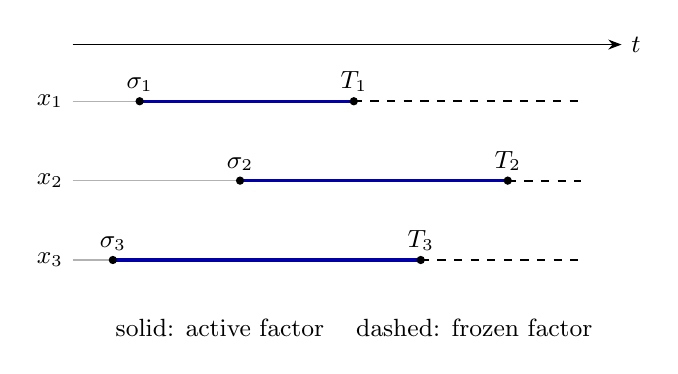
\begin{tikzpicture}[x=0.85cm,y=0.72cm,>=Stealth,font=\small]
  \draw[->] (0,1) -- (8.2,1) node[right] {$t$};
  \foreach \y/\i/\start/\finish in {0/1/1/4.2,-1.4/2/2.5/6.5,-2.8/3/0.6/5.2} {
    \node[left] at (0,\y) {$x_{\i}$};
    \draw[gray!60] (0,\y)--(\start,\y);
    \draw[very thick,blue!65!black] (\start,\y)--(\finish,\y);
    \draw[dashed,thick] (\finish,\y)--(7.6,\y);
    \fill (\start,\y) circle(1.5pt);
    \fill (\finish,\y) circle(1.5pt);
    \node[above] at (\start,\y) {$\sigma_{\i}$};
    \node[above] at (\finish,\y) {$T_{\i}$};
  }
  \node[align=center] at (2.2,-4) {solid: active factor};
  \node[align=center] at (6,-4) {dashed: frozen factor};
\end{tikzpicture}
\caption{The multipoint event uses each point's own activation and target
stop. The solid intervals may overlap in any order. After $T_i$ the
factor for $x_i$ is constant, and no further survival of that point is
required. The axis is schematic physical time, not the individual
conformal-radius clocks.}
\label{fig:individual-stops}
\end{figure}


Put $Q=\prod_{i=1}^m Q_i$. If all points finish, this product has
the deterministic value
\[
 Q=3^{-m}\prod_i(b_i/e_i)^\alpha.
\]
Thus a uniform bound on the expectation of a discounted product will
give the desired probability estimate, provided the total discount is
deterministically bounded. The individual negative drifts absorb
the singular angular terms, and the pair interaction estimate pays for
what remains. We give both estimates explicitly. Write
$s=\sin\theta$, $k=q(p-q)/2$, and $\sigma=\delta'/\delta$, so
$|\sigma|\le\beta\le1$ almost everywhere. Formula~\eqref{op:sine-generator}
gives
\begin{equation}
 \frac{(\partial_u+\mathcal L+p/2)f}{f}
 =\frac\delta f\left[
 \frac p2+\frac{(p-q)(1+q)}2s^q-ks^{q-2}
                         +\sigma(1+s^q)\right].
 \label{mp:exact-drift}
\end{equation}
Let
\[
 A=\frac p2+\frac{(p-q)(1+q)}2+2,
 \qquad h_0=\left(\frac{k}{2A}\right)^{1/(2-q)}\in(0,1).
\]
The bracket in \eqref{mp:exact-drift} is at most $A-ks^{q-2}$.
For $s<h_0$, adding $(k/2)D$ leaves a nonpositive expression.
For $s\ge h_0$, use $f\ge s^p\ge h_0^p$. We obtain
\begin{equation}
 \frac{(\partial_u+\mathcal L+p/2)f}{f}
 \le C_1\delta-c_1D,
 \qquad C_1=Ah_0^{-p},\quad c_1=k/2>0.
 \label{mp:drift-bound}
\end{equation}
All these constants depend only on $a$. The corner of $\delta$ at
$U_i/2$ causes no additional term: it is an absolutely continuous
function of the finite-variation clock $u_i$.

Because $q<p$, $q<1$, and $0<\delta\le1$, angular differentiation
gives $|\partial_\theta f|\le(p+q)s^{q-1}$. Also $\delta\le f\le3$,
and $\eta(q-2)=q-1$. Therefore
\begin{equation}
 \frac{|\partial_\theta f|}{f}
 \le(p+q)\delta^{-1}s^{q-1}
 \le(p+q)3^\eta\delta^{-1-\eta}D^\eta.
 \label{mp:derivative-bound}
\end{equation}
This bound includes the singular angular behavior when $p<1$.

On active intervals, the normalized
Brownian coefficient of $Q_i$ is
$(\partial_\theta f_i/f_i)V_i$. It\^o's Product Formula thus gives
one cross term for each unordered active pair. Its absolute value is
bounded, by \eqref{mp:derivative-bound}, by
\[
 C_2(\delta_i\delta_j)^{-1-\eta}
    (D_iV_i^2)^\eta(D_jV_j^2)^\eta(V_iV_j)^{1-2\eta}.
\]
Weighted Young's Inequality with weights $\eta,\eta,1-2\eta$ shows
that for any $\epsilon>0$ this is at most
\begin{equation}
 \epsilon(D_iV_i^2+D_jV_j^2)
       +C_\epsilon(\delta_i\delta_j)^{-M}V_iV_j.
 \label{mp:young}
\end{equation}
Indeed, putting $r=1-2\eta$, the weighted arithmetic--geometric
mean inequality gives the displayed bound with
$C_\epsilon=rC_2^{1/r}(\eta/\epsilon)^{2\eta/r}$, and raises
$\delta_i\delta_j$ to exponent $-(1+\eta)/r=-M$.
For $m>1$ choose $\epsilon=c_1/[2(m-1)]$; for $m=1$ there are no
cross terms. Summing \eqref{mp:drift-bound} and \eqref{mp:young}
absorbs the pair contributions into the negative terms. A nonnegative
upper bound for the remaining normalized physical-time drift is
\[
 k_t=C_1\sum_{i\text{ active}}\delta_iV_i^2
       +C_3\sum_{\substack{i<j\\i,j\text{ active}}}
                     (\delta_i\delta_j)^{-M}V_iV_j,
\]
where $C_3$ depends only on $m,a$ (and the pair sum is zero for $m=1$).
Its total integral has a deterministic bound. Namely,
\[
 \int_0^{U_i}\delta_i(u)\,\dd u
 =\frac2\beta(1-e^{-\beta U_i/2})\le\frac2\beta,
 \qquad
 (\delta_i\delta_j)^{-M}\le e^{M\beta(u_i+u_j)}.
\]
Equation~\eqref{mp:interaction-integral}, with $c=M\beta$, yields
\begin{equation}
 \int k_t\,\dd t\le
 K_{m,a}:=\frac{2mC_1}{\beta}
             +C_3\binom m2 I(a,M\beta)<\infty.
 \label{mp:discount}
\end{equation}
It follows that
$Q_t\exp(-\int_0^t k_v\,\dd v)$ is a nonnegative local
supermartingale on every nonsingular interval, including its downward
activation and completion jumps.

\begin{proof}[Completion of the proof of Proposition~\ref{mp:estimate}]
To justify stopping the product, monitor \emph{all unfinished points},
including those not yet active. Stop if any of their angles leaves
$(1/N,\pi-1/N)$, if any of their heights $Y_i$ falls to $1/N$, or at
physical time $N$. Denote this cutoff by $\zeta_N$, and also stop when
all targets have been completed. No cutoff is imposed on a completed
point. At these stops every stochastic integral used above is
legitimate; a further standard bounded localizer, followed by Fatou,
gives expectation at most the initial value, which is at most $1$.
There is no need to continue a factor through the singular lifetime of
an unsuccessful unfinished point.

Put $T_{\rm all}=\max_iT_i$. On $\{T_{\rm all}<\zeta_N\}$, the final
discounted product is at least
\[
 e^{-K_{m,a}}3^{-m}\exp\left(\frac p2\sum_iU_i\right).
\]
Consequently
\[
 \PP(T_{\rm all}<\zeta_N)
 \le 3^m e^{K_{m,a}}
                   \exp\left(-\frac p2\sum_iU_i\right).
\]
Every successful path belongs to these events for all sufficiently
large $N$. Indeed, each point remains alive through its own finite
$T_i$, so its continuous height and its distance in angle from the
endpoints have strictly positive minima on $[0,T_i]$. There are only
finitely many points, and later swallowing of a finished point is
irrelevant. Thus cutoff exhaustion covers precisely all the success
paths needed for the upper bound. Since $p/(4a)=\alpha$, passage to
the limit gives \eqref{mp:hit-bound} with
$C_{m,a}=3^m e^{K_{m,a}}$ when all $e_i<b_i$.

For equality targets, or targets larger than their caps, retain only
the strict constraints $e_i<b_i$. The original event is contained in
the retained event, and all separation assumptions still hold.
Taking the maximum of the constants for at most $m$ retained points,
including the empty set, proves \eqref{mp:capped-hit-bound} and the
full stated proposition.
\end{proof}

\paragraph{Comparison with the Euclidean estimate.}
To deduce the proposition from Rezaei--Zhan, put $f=J^{-1}$,
$z_i=f(x_i)$, $\lambda_i=|f'(x_i)|$, and $z_0=0$.
Koebe's Quarter Theorem applied to $f$ on $B(x_i,b_i/4)\subset D$
gives
\begin{align*}
 |z_i-z_j|&\ge\lambda_i b_i/16
                   &&(1\le j\le m,\ j\ne i),\\
 \operatorname{Im}z_i
 &=\lambda_iR_D(x_i)/2\ge\lambda_i b_i/2.
\end{align*}
Indeed, $f(B(x_i,b_i/4))$ contains the disk with center $z_i$ and
radius $\lambda_i b_i/16$, whereas every other $x_j$ lies outside
$B(x_i,b_i/4)$. Retain only targets with $e_i<b_i/32$ and relabel
the retained points; if none remain, the trivial probability bound
suffices. Their preceding-point distances satisfy
$l_i=\min_{0\le j<i}|z_i-z_j|\ge\lambda_i b_i/16$.
At a successful hit, radius covariance gives
$R_{H_t}(z_i)=\lambda_i e_i$. Koebe's distance
bound then puts the past half-plane trace within
$r_i=\lambda_i e_i$ of $z_i$: the real line is farther away.
Theorem~1.1 and equation~(1.5) of \cite{RezaeiZhan2017} give
\[
 \PP\{\dist(z_i,\gamma)\le r_i\text{ for all retained }i\}
 \le C_{m,a}\prod_{i\text{ retained}}(r_i/l_i)^\alpha
 \le C_{m,a}16^{m\alpha}
             \prod_{i\text{ retained}}(e_i/b_i)^\alpha.
\]
Each omitted target contributes at least $32^{-\alpha}$ to the capped
product, so it can
be restored by enlarging the constant. This proves the stated
domain-uniform consequence without a boundary extension of $J$.

\subsection{Integrating the collision singularities}

\begin{lemma}[Capped distance kernels]\label{mp:kernel-integral}
Let $0<\alpha<1$, $b>0$, and let $K\subset\mathbb C$ be a bounded Borel set.
For distinct $x_1,\ldots,x_m$ set
\[
 b_i=\min\bigl(b,\min_{j\ne i}|x_i-x_j|\bigr),\qquad
 F_b(x_1,\ldots,x_m)=\prod_{i=1}^m b_i^{-\alpha},
\]
where the inner minimum is omitted when $m=1$. Then
\begin{equation}
 \int_{K^m}F_b(x_1,\ldots,x_m)\prod_i\dd A(x_i)<\infty.
 \label{mp:all-variable-integral}
\end{equation}
The same assertion holds with one point fixed: for bounded $K_0$,
\begin{equation}
 \sup_{x_0\in K_0}\int_{K^m}
 F_b(x_0,x_1,\ldots,x_m)\prod_{i=1}^m\dd A(x_i)<\infty.
 \label{mp:fixed-center-integral}
\end{equation}
Values on diagonals may be set to infinity; they do not affect these
integrals.
\end{lemma}

\begin{proof}
For each factor,
$b_i^{-\alpha}\le b^{-\alpha}+\sum_{j\ne i}|x_i-x_j|^{-\alpha}$.
Expand their product. Each resulting term corresponds to a directed
graph with at most one outgoing edge per vertex, no self-edge, and a
factor $|x_i-x_j|^{-\alpha}$ for each edge $i\to j$.
Integrate a vertex with no incoming edge: if it has one outgoing
edge its integral is bounded uniformly in the other endpoint because
$\alpha<2$; if isolated it contributes only the area of a containing
box. Repeating removes all trees attached to directed cycles and all
components without cycles.

For a remaining cycle of length at least three, one vertex has two
incident factors. Their integral is uniformly bounded by
\[
 \int_K|x-y|^{-\alpha}|x-z|^{-\alpha}\,\dd A(x)
 \le\left(\int_K|x-y|^{-2\alpha}\,\dd A(x)\right)^{1/2}
      \left(\int_K|x-z|^{-2\alpha}\,\dd A(x)\right)^{1/2}
 \le C_K,
\]
since $2\alpha<2$. Removing this vertex leaves a chain, whose
endpoints can be integrated successively. A two-cycle contributes
$|x-y|^{-2\alpha}$, so the same integrability applies directly.
There are finitely many graph terms, proving
\eqref{mp:all-variable-integral}.

For the fixed point, choose $R<\infty$ such that
$K-x_0\subset B(0,R)$ for every $x_0\in K_0$. The kernel $F_b$ is
invariant under simultaneous translation, with the cap $b$ unchanged.
Thus the integral in \eqref{mp:fixed-center-integral} is bounded by
\[
 \int_{B(0,R)^m}F_b(0,y_1,\ldots,y_m)\prod_i\dd A(y_i).
\]
Average a simultaneous translation by $v\in B(0,1)$. A change of
variables bounds the last display by
\[
 \frac1{|B(0,1)|}
 \int_{B(0,R+1)^{m+1}}F_b(v,x_1,\ldots,x_m)
                       \,\dd A(v)\prod_i\dd A(x_i),
\]
which is finite by the already proved assertion. This is translation
invariance of a deterministic distance kernel; no translation
invariance of a chordal SLE law is required.
\end{proof}

We record precisely the moment consequence used in the next sections.
For $l>0$ let
\[
 A_l(\dd x)=G_{\tau_l(x)}(x)
                       \ind_{\{\tau_l(x)<\infty\}}\,\dd A(x).
\]

\begin{corollary}[Integrated level weights]\label{mp:level-moments}
Let $f\ge0$ be bounded and supported in a compact $K\Subset D$.
Then, for every integer $m\ge1$,
\begin{equation}
 \sup_{l>0}\EE[A_l(f)^m]<\infty.
 \label{mp:ordinary-moments}
\end{equation}
Fix also $x_0\in D$ and $0<e_0\le R_D(x_0)$, and let $E_0$ be the
event that $x_0$ reaches radius $e_0$ while alive. Then
\begin{equation}
 \sup_{l>0}\EE[\ind_{E_0} A_l(f)^m]\le C e_0^\alpha.
 \label{mp:center-moments}
\end{equation}
Here $C$ can be chosen using only $m,a$, the size and support of $f$,
the bounded location of $x_0$, and a positive lower bound for
$R_D$ on $K\cup\{x_0\}$. In particular, in a fixed disk these bounds
are uniform over all initial boundary angles.
\end{corollary}

\begin{proof}
Choose a fixed cap $b>0$ below the indicated initial radii, and cap
it further by nearest-neighbor distances for each integration tuple.
At point $x_i$, the target is $e_i=R_D(x_i)e^{-2al}$, and
$G_{\tau_l(x_i)}(x_i)\le e_i^{-\alpha}$ on success. Tonelli and
\eqref{mp:capped-hit-bound} therefore bound the $m$th moment by
\[
 C_{m,a}\int_{K^m}\prod_{i=1}^m f(x_i)b_i^{-\alpha}
                                                 \prod_i\dd A(x_i),
\]
because $e_i^{-\alpha}\min\{1,(e_i/b_i)^\alpha\}\le b_i^{-\alpha}$.
This proves \eqref{mp:ordinary-moments} by
Lemma~\ref{mp:kernel-integral}. For the additional fixed center, apply
the same argument to $m+1$ points and use
\[
 \min\{1,(e_0/b_0)^\alpha\}\le e_0^\alpha b_0^{-\alpha}.
\]
The fixed-center integral proves \eqref{mp:center-moments}, even
when the center's target exceeds its distance cap. No relative order
of the center hit and the other hits is imposed. Finally, in $\DD$
one has $R_D(x)=1-|x|^2$, independently of its boundary marks. The
proof was carried out directly in the physical domain, so a
degenerating half-plane identification introduces no additional
constant.
\end{proof}

\section{A canonical mass on the trace}
\label{mass:section}

We now turn the Green potential into an increasing measure on the trace.
The conditional Green-potential approach goes back to
Lawler--Sheffield \cite[Proposition~2.2 and Section~3]{LawlerSheffield2011}
and Lawler--Zhou \cite[Proposition~A and Theorem~1]{LawlerZhou2013};
see also the Minkowski-content construction in \cite{LawlerRezaei2015}.
Here one common sequence of convex combinations supplies the mass and
all of its versions. We construct the measure and prove the
properties needed below directly; no identification with Minkowski content
is required.  All measures in this section are measures on the open domain.
Write $\lambda(f)=\int f\,\dd\lambda$ for integration against a measure.

\begin{proposition}[Construction and conditional kernel]
\label{mass:construction}
There is an adapted increasing family $(\mu_t)_{0\le t\le\infty}$ of
locally finite measures on $\HH$, starting at zero, with the following
properties.  Its terminal measure is nonatomic and has moments of every
integer order on compact sets.  Almost surely, simultaneously for all
$0\le v<t<\infty$, the increment $\mu_t-\mu_v$ is carried by
$\gamma([v,t])\cap\HH$.  The process is locally continuous in total
variation, and $\mu_t\uparrow\mu_\infty$ as $t\to\infty$.
For every stopping time $S$, possibly infinite,
\begin{equation}
 \EE\bigl[\mu_\infty(\dd x)-\mu_S(\dd x)\mid\mathcal F_S\bigr]
   =G_S(x)\,\dd A(x),
 \qquad G_\infty:=0.
 \label{mass:kernel}
\end{equation}
This is an equality of conditional measure kernels; in particular it
allows nonnegative tests known at time $S$.  Moreover,
\begin{equation}
 \EE\mu_\infty(\dd x)=G_0(x)\,\dd A(x).
 \label{mass:mean}
\end{equation}
\end{proposition}

\subsection{Deterministic convex extraction}

The compact moment bounds permit one simultaneous limit for all
rational times and a determining family of spatial tests. Keeping the
same convex coefficients is what later makes the kernels and conformal
images properties of one measure rather than separately chosen versions.

For an integer $j\ge1$ define
\begin{equation}
 M_t^{(j)}(\dd x)
 =G_{\tau_j(x)}(x)
   \ind_{\{\tau_j(x)\le t,\ \tau_j(x)<\infty\}}\,\dd A(x),
 \qquad 0\le t\le\infty.
 \label{mass:approximants}
\end{equation}
The density is zero on failure to reach the level.  For a compact
$C\Subset\HH$, fix $c_C>0$ with $c_C\le\inf_C R_0$.  Given distinct
$x_1,\ldots,x_m\in C$, set
\[
 b_i=\min\bigl(c_C,\min_{k\ne i}|x_i-x_k|\bigr),
\]
where the second minimum is omitted when $m=1$.
The terminal approximant is the level weight $A_j$ of
Corollary~\ref{mp:level-moments}.  The collision-kernel estimate in its
proof gives, for every bounded nonnegative $f$ supported in $C$,
\begin{equation}
 \sup_j\EE\bigl[M_\infty^{(j)}(f)^m\bigr]
 \le C_{m,a}\int_{C^m}
       \prod_{i=1}^m f(x_i)b_i^{-\alpha}
       \,\dd A(x_1)\cdots\dd A(x_m)<\infty.
 \label{mass:moment-bound}
\end{equation}
The last assertion is Lemma~\ref{mp:kernel-integral}.
All constants are independent of $j$.

We obtain one sequence of convex combinations as follows.  Choose a
countable family of continuous compactly supported tests, uniformly
dense among tests supported in each member of a compact exhaustion.
Include nonnegative cutoff functions equal to one on that exhaustion,
and rational linear combinations of the chosen tests.  Enumerate the
pairs of these tests with times in $\mathbb Q_+\cup\{\infty\}$ as
$(f_r,t_r)$, $r\ge1$, and set
$X_r^{(j)}=M_{t_r}^{(j)}(f_r)$.
Each coordinate is bounded in $L^2$ by \eqref{mass:moment-bound}.
A diagonal subsequence $j_l$ has a weak limit $X_r$ in every coordinate.

For each $k$, consider the first $k$ coordinates as a vector in
$(L^2)^k$.  Its weak limit $(X_1,\ldots,X_k)$ lies in the norm closure
of the convex hull of every tail.  Hence there are deterministic
coefficients $c_{kl}\ge0$, supported on finitely many $l\ge k$, with
$\sum_lc_{kl}=1$, such that
\[
 \sum_{r=1}^k\left\|
       \sum_{l\ge k}c_{kl}X_r^{(j_l)}-X_r
                    \right\|_2^2\le4^{-k}.
\]
Define
\[
 \overline M_t^{(k)}=\sum_{l\ge k}c_{kl}M_t^{(j_l)}.
\]
For every listed pair, the summable squared errors give both $L^2$
and almost-sure convergence; intersecting the resulting events over
$r$ gives simultaneous convergence on the whole countable list.
The same coefficient row is used for every time and spatial test.

On this event, the cutoff tests bound all local masses.  Density therefore
extends convergence to every continuous compactly supported test.
The limiting positive functionals are Radon measures, with almost-sure
vague convergence at all listed times.  Positivity and ordering in time
pass to the limit.  The limits at finite rational times are adapted, since
the corresponding $L^2(\mathcal F_t)$ subspaces are closed.  Convexity and
Fatou's Lemma preserve \eqref{mass:moment-bound} for the terminal measure
and continuous nonnegative tests.  Approximation then gives the compact
moment assertions.

We also obtain nonatomicity, which will be needed to pass from rational
times to all times.  For two points in a fixed larger compact the kernel
in \eqref{mass:moment-bound} is bounded by
$C(1+|x-y|^{-2\alpha})$.  Cover a given smaller compact by mesh squares
of side $\delta$, and majorize each square's indicator by a continuous
cutoff in a slightly enlarged square.  The enlarged squares have bounded
overlap.  The expected sum of their squared masses is bounded by
\[
 C\iint_{|x-y|\le C\delta}
       (1+|x-y|^{-2\alpha})\,\dd A(x)\dd A(y),
\]
where both variables lie in the larger compact.  This tends to zero
because $2\alpha<2$.  Every atom in the smaller compact contributes the
square of its mass to the corresponding sum at every mesh size.
Fatou's Lemma, followed by a countable compact exhaustion, proves that
$\mu_\infty$ has no atoms.

\subsection{Support, continuity, and stopping times}

The finite-level conditional weight identity of
Lemma~\ref{op:finite-tilt} gives, at a finite rational time $t$,
\begin{equation}
 \EE\bigl[M_\infty^{(j)}(\dd x)-M_t^{(j)}(\dd x)
             \mid\mathcal F_t\bigr]
 =G_t(x)\ind_{\{x\in H_t,\ R_t(x)>R_0(x)e^{-2aj}\}}\,\dd A(x).
 \label{mass:approx-kernel}
\end{equation}
The strict inequality excludes a level already attained at $t$.
At every surviving point the indicator tends to one.  Since
$\EE G_t(x)\le G_0(x)$, dominated convergence on compact tests applies to
the right side.  Local $L^2$ bounds give uniform integrability on the
left.  Passing through the tail convex combinations proves
\eqref{mass:kernel} at rational times.  The mean-one finite-level weights
also give \eqref{mass:mean}.

These identities initially hold for countably many deterministic tests.
They identify the conditional measure kernel, and hence, by the Monotone
Class Theorem, hold against every nonnegative
$\mathcal F_t\otimes\mathcal B(\HH)$-measurable test.  In particular,
testing the complement of the known surviving domain shows that
\begin{equation}
 \mu_\infty-\mu_t\text{ is carried by }H_t
 \quad\text{at every finite rational }t,
 \label{mass:future-support}
\end{equation}
on one event of probability one.

At the same times, $\mu_t$ is carried by the past trace.  Indeed, on a
fixed compact, a point receiving mass in $M_t^{(j)}$ has, at its level
time, distance at most $R_0(x)e^{-2aj}$ from the current domain boundary.
For large $j$ that nearby boundary cannot be the real line, so it belongs
to $\gamma([0,t])$.  Thus the approximants, and their tail convex
combinations, are carried locally by shrinking neighborhoods of this
closed trace segment.  Vague convergence gives the claimed support.
For rational $v<t$, the increment is dominated by $\mu_t$ and by
$\mu_\infty-\mu_v$, so it is carried by $\gamma([v,t])\cap\HH$.

Take increasing rational left limits and decreasing rational right limits
of the measure process.  At any finite time $w$, their difference is
dominated by increments over every rational interval containing $w$.
Continuity of the trace forces its support to lie in the singleton
$\{\gamma(w)\}\cap\HH$.  The difference vanishes by nonatomicity.
At zero use zero as the left limit; the same argument gives zero, since
$\gamma(0)\notin\HH$.  This argument is pathwise on the one event already
constructed and therefore works simultaneously for every $w$.
It defines an increasing process on all times, locally continuous in total
variation: on a compact the variation of a positive increment is just its
mass, and the possible one-sided jump measures have been shown to vanish.
Adaptedness follows from the rational left limits.
The support assertion for arbitrary intervals follows by enclosing them
in rational intervals and taking limits.

The terminal value is exhausted by finite times.  By
Proposition~\ref{op:potential}, $\EE G_t(x)\to0$ as $t\to\infty$.
Apply \eqref{mass:kernel} at integer times and use
$\EE G_t\le G_0$ on compact tests.  The nonnegative measure
$\mu_\infty-\lim_{t\to\infty}\mu_t$ has zero mean, and hence is zero.
This also gives local total-variation convergence at infinity.

For completeness, let $S$ be any stopping time.  On the event of rational
convergence, monotonicity squeezes $\overline M_S^{(k)}(f)$ between its
values at rational times approaching each realized finite $S$.
Continuity gives convergence to $\mu_S(f)$ for every nonnegative
continuous compact test.  On $\{S=\infty\}$ use terminal convergence of
the extracted sequence.  Uniform integrability again follows from the
terminal $L^2$ bound.  The finite-level identity
\eqref{mass:approx-kernel} holds with $t$ replaced by $S$, and with zero
right side on $\{S=\infty\}$.  The bound
$\EE[G_S(x);S<\infty]\le G_0(x)$ from
Proposition~\ref{op:potential} permits the same dominated convergence.
This proves \eqref{mass:kernel} at $S$, including its conditional-kernel
interpretation, and completes Proposition~\ref{mass:construction}.

\begin{corollary}[First-visit accounting]
\label{mass:first-visit}
Put $v(x)=\inf\{t\ge0:\gamma(t)=x\}$, with value infinity if the set is
empty.  Almost surely $v(x)<\infty$ for $\mu_\infty$-almost every $x$, and
simultaneously for every finite $t$,
\begin{equation}
 \mu_t(\dd x)=\ind_{\{v(x)\le t\}}\mu_\infty(\dd x).
 \label{mass:first-visit-identity}
\end{equation}
\end{corollary}

\begin{proof}
At rational $t$, past mass is carried by $\gamma([0,t])$, while remaining
mass is carried by the open set $H_t$, disjoint from that past trace.
This proves the identity there.  Increasing finite times exhaust the
terminal measure.  Right approximation by rational times, continuity of
the measure process and of the trace, then proves the identity at all
times.  In particular a later geometric return to an already visited
point introduces no new mass there.
\end{proof}

\subsection{Versions, conformal maps, and restart}

We have constructed the continuous mass and its conditional kernel.
To use them at centered stops and in random future domains, we next
fix a measurable path functional and establish equality of the actual
restarted measures.

We fix one nonanticipating measurable version of this construction.
On the canonical continuous-path space each $M^{(j)}$, tested on an
interior compact, is a raw adapted c\`adl\`ag process: its terminal density
has a deterministic finite bound there, and one-sided continuity follows
from dominated convergence of the hitting-time indicators.
The same holds for every deterministic convex combination.
At each finite time, take the vague limit of $\overline M_t^{(k)}$
where it exists, and use the zero measure otherwise.  The space of
locally finite positive Radon measures is Polish in the vague topology;
its convergence set and limit map are therefore Borel.  This defines
a raw progressively measurable measure-valued functional.  At infinity use the same limit rule for
$\overline M_\infty^{(k)}$.  Rational squeezing as above shows that it
agrees, simultaneously at every time under the ordinary Brownian law,
with the continuous process just constructed.

All evaluations under a centered law use this raw functional of the
stopped path.  At each finite inner level the density in
Lemma~\ref{op:finite-tilt} transfers the required statements about
that stopped piece.  Consistent laws of the stopped pieces, and increasing
limits of their coordinates, suffice thereafter.  We do not extend the
centered law to the original Brownian space completed by infinite-future
null sets.  This distinction also ensures parameter measurability:
Loewner solutions, level times and conformal maps are measurable in the
driver and marked point, and progressive evaluation of the fixed mass
functional at those times is measurable.

For a fixed conformal identification $J:\HH\to D$, define
\begin{equation}
 \mu_t^D=J_*\bigl(|J'|^d\mu_t\bigr).
 \label{mass:conformal}
\end{equation}
This rule holds exactly for the approximants: conformal radius contributes
$|J'|^{-\alpha}$ and area contributes $|J'|^2$, so their product is
$|J'|^d$.  Inner-clock ratios are unchanged.
A compact continuous test in $D$ pulls back to such a test in $\HH$.
Thus the same deterministic convex combinations converge in every fixed
image domain, on the event giving convergence for all compact continuous
tests.  The kernel, local continuity, nonatomicity and support statements
hold there with the corresponding $G_t^D$. More precisely, its increments
are carried by $J(\gamma([v,t])\cap\HH)$. The map is applied only to
interior trace points; an arbitrary $J$ need not extend continuously
to the boundary.
The construction is jointly measurable in a measurable family of maps
$J$; it requires no new extraction for different maps.

The kernel also proves uniqueness.  If $A_t$ and $\widetilde A_t$ are
two continuous increasing adapted test-mass processes starting at zero,
with integrable terminal values and the same remaining conditional
potential, then
\[
 A_t-\widetilde A_t
   =\EE[A_\infty-\widetilde A_\infty\mid\mathcal F_t].
\]
Their difference is a continuous martingale of finite variation, hence
vanishes.  Applying this to a countable determining set of tests proves
uniqueness of the measure process.  In particular it removes dependence
on the convex extraction.  It also gives Brownian scaling: if
$B^{(c)}_t=c^{-1}B_{c^2t}$, then, for each $c>0$,
\begin{equation}
 \mu_t(B^{(c)})(A)=c^{-d}\mu_{c^2t}(B)(cA)
 \quad\text{almost surely, for all }t\text{ and Borel }A\subset\HH.
 \label{mass:scaling}
\end{equation}
Indeed the scaled process has the same kernel, continuity and terminal
integrability as the canonical process for $B^{(c)}$.

For natural parametrization, Lawler--Rezaei
\cite[Proposition~3.13]{LawlerRezaei2012Basic} prove conformal restart
at an almost surely finite stopping time, simultaneously over later
time intervals.  We prove the following measure-valued identity for
the mass constructed here directly from its conditional kernel.

\begin{proposition}[Pathwise interior restart]
\label{mass:restart}
Fix a stopping time $S$.  On $\{S<\infty\}$ put
$J_S=(g_S-B_S)^{-1}:\HH\to H_S$, and let $\widetilde\mu$ be the canonical
mass functional of the fresh Brownian motion $B_{S+t}-B_S$.
Almost surely, as measures on $H_S$, simultaneously for all
$0\le t\le\infty$,
\begin{equation}
 (\mu_{S+t}-\mu_S)|_{H_S}
       =(J_S)_*\bigl(|J_S'|^d\widetilde\mu_t\bigr).
 \label{mass:restart-identity}
\end{equation}
The same assertion holds when the initial domain is a fixed conformal
image of $\HH$.  Once this equality of measures has been obtained,
one may integrate any random nonnegative Borel weight on the restart
domain and evaluate at any later random time.
\end{proposition}

\begin{proof}
Write $\nu_t$ for the right side of \eqref{mass:restart-identity} on
$\{S<\infty\}$, and set both processes in the comparison below to zero
on $\{S=\infty\}$.  Take a countable collection of rational balls
$U\Subset\HH$, and dense
countable families of nonnegative tests $\phi\in C_c(U)$, including local
cutoffs.  Localize each comparison to
\[
 E_U=\{S<\infty,\ \overline U\subset H_S\}\in\mathcal F_S.
\]
We first check terminal integrability, before invoking uniqueness.
Conditioning on $\mathcal F_S$, the strong Markov property, the canonical
mean measure and change of variables give
\begin{equation}
 \EE[\ind_{E_U}\nu_\infty(\phi)\mid\mathcal F_S]
       =\ind_{E_U}\int\phi(x)G_S(x)\,\dd A(x).
 \label{mass:restart-integrability}
\end{equation}
The pulled-back test is random, with potentially random derivative and
support bounds.  The formula remains valid: first use nonnegative simple
functions of the restart data and source point, and then apply conditional
Tonelli and monotone convergence.  Its expectation is at most
$\int\phi G_0\,\dd A<\infty$.  Thus the candidate terminal test mass is
integrable.  The actual terminal increment is bounded by
$\mu_\infty(\phi)$ and is integrable as well.

At $S+t$, the candidate and actual increment have the same remaining
conditional potential.  For the candidate, this follows from the
canonical kernel for the fresh driver, with its $\mathcal F_S$-measurable
pulled-back test; the Loewner composition rule and
\eqref{mass:conformal} transform that potential into $G_{S+t}$.
For the actual process it is \eqref{mass:kernel} at $S+t$.
Consequently
\[
 D_t:=\ind_{E_U}\bigl[(\mu_{S+t}-\mu_S)(\phi)-\nu_t(\phi)\bigr]
       =\EE[D_\infty\mid\mathcal F_{S+t}].
\]
This continuous finite-variation martingale starts at zero and is
identically zero.  Intersect the resulting events over the countable
balls and tests, and use continuity to obtain equality for all times.
Those balls whose closures lie in the realized $H_S$ cover it; their
tests determine its locally finite measures.  This proves the pathwise
measure equality throughout the random domain.

Only now do we integrate random weights.  In particular, if
$F:\DD\to H_S$ is a random conformal map and $K\Subset\DD$, the Borel
weight
\[
 \ind_{F(K)}(x)\,|F'(F^{-1}(x))|^{-d}
\]
is bounded on its realized compact support.  Its integration follows
directly from equality of the realized measures, without a further
exceptional event indexed by $F$ or $K$.  The all-time equality similarly
permits substitution of a later random time.  Composition with a fixed
initial identification proves the last domain assertion.
\end{proof}

To obtain the centered restart rule, first work under the ordinary law.
For a stopping time $S$, work on $\{S<\infty,\ z\in H_S\}$ and write
$g_S(z)-B_S=\lambda e^{i\theta}$, where $\lambda>0$.
Conditionally on $\mathcal F_S$, the rescaled fresh driver
$\lambda^{-1}(B_{S+\lambda^2u}-B_S)$ is standard Brownian motion.
We may apply \eqref{mass:scaling} at this random scale: after conditioning,
$\lambda$ is fixed, the fresh driver is independent of $\mathcal F_S$,
and the scaling equality holds almost surely at each fixed scale.
Joint measurability of the mass functional permits this conditioning.
Together with Proposition~\ref{mass:restart}, scaling identifies the
actual future mass in these coordinates.

Now apply the finite change of law through the next radius target of
$z$.  The ratio of Green weights is conformally invariant, since the
derivative at the marked point cancels between the two weights.
Lemma~\ref{op:finite-tilt} therefore identifies, conditionally on the
stopped past under the centered law, the future mass pulled back to a
disk centered at $z$ with the canonical disk law of starting angle
$\theta$.  This assertion uses only data through the finite test endpoint.

\begin{proposition}[Positive mass on every interval]
\label{mass:positive}
Almost surely, for every \mbox{$0\le v<t<\infty$},
\[
 (\mu_t-\mu_v)(\HH)>0.
\]
The positive mass can always be detected on an interior compact.  The
same statement holds in every fixed conformal image, in its associated
half-plane time.
\end{proposition}

\begin{proof}
Equation~\eqref{mass:mean} gives positive terminal expectation on a
compact with nonempty interior.  Terminal exhaustion therefore gives
positive probability of positive interior mass by some finite
deterministic time.  Scaling shows that
$\PP\{\mu_t(\HH)>0\}$ has the same positive value for every $t>0$.
The raw event $\limsup_{n\to\infty}\{\mu_{1/n}(\HH)>0\}$ belongs
to the Brownian germ sigma field. On the common event of monotonicity it
equals $\bigcap_{n\ge1}\{\mu_{1/n}(\HH)>0\}$, so has this same
probability. The germ zero--one law
makes it one.  Hence positive mass is present before every positive time.
Restart at each rational time and apply
Proposition~\ref{mass:restart}.  The strictly positive conformal weight
preserves positivity, giving positive increments on all rational
intervals on one event.  Every nontrivial real interval contains a
nontrivial rational interval.  A countable compact exhaustion detects
the positive increment mass; \eqref{mass:conformal} proves the image-domain
assertion.
\end{proof}

\section{Disk moments and deterministic coefficients}
\label{coef:section}

We now supply the deterministic numbers that select the gauge. First,
the physical-domain multipoint estimate proves that one centered disk
mass has positive finite moments. Then its conditional Green potential
recovers those moments through an explicit sequence of integrals.
The last subsection realizes the integrands by normal coordinates and
ordinary differential equation limits.

\subsection{The centered disk model}

For $0<\theta<\pi$, use the conformal identification
$J_\theta:\HH\to\DD$ below.  It takes $e^{i\theta}$ to the marked center
$0$.  Denote the ordinary law in these coordinates by $\PP_\theta$, and
its centered finite-level laws at $0$ by $\PP_\theta^*$.
Average the latter over the invariant angle law $\pi_a$, and write
$\PP_{\mathrm{mix}}^*$ for the resulting consistent stopped laws.
Define
\begin{equation}
 \begin{gathered}
 J_\theta(\zeta)=\frac{\zeta-e^{i\theta}}{\zeta-e^{-i\theta}},
 \qquad K=\{x\in\DD:|x|\le\tfrac14\},
 \qquad \PP_{\mathrm{mix}}^*=\int_0^\pi\PP_\theta^*\,\pi_a(\dd\theta),
 \\
 L_\ell=\mu^{\DD}_{\tau_\ell(0)}(K),
 \qquad L=\lim_{\ell\to\infty}L_\ell.
 \end{gathered}
 \label{coef:disk-model}
\end{equation}
The disk mass is the weighted pushforward of the single canonical
half-plane functional in Section~\ref{mass:section}.
Each $L_\ell$ is a raw finite-stopped-path quantity; its increasing limit
is defined on the consistent collection of such quantities.  In
particular \eqref{coef:disk-model} does not require a Brownian
continuation after the centered terminal time.

\begin{proposition}[Finite, positive disk moments]\label{coef:positive-moments}
For every integer $n\ge1$, the deterministic numbers
\begin{equation}
 m_n(\ell):=\EE_{\mathrm{mix}}^*L_\ell^n,
 \qquad
 m_n:=\EE_{\mathrm{mix}}^*L^n
       =\lim_{\ell\to\infty}m_n(\ell)
       \quad\text{satisfy}\quad 0<m_n<\infty.
 \label{coef:moments}
\end{equation}
Moreover $L>0$ almost surely, and, for each fixed angle,
\begin{equation}
 \sup_{\ell>0}\EE_\theta^*L_\ell^n
                  \le C_{n,a}\sin^{-p}\theta.
 \label{coef:angle-moments}
\end{equation}
\end{proposition}

\begin{proof}
We apply the multipoint estimate directly in the physical disk.
Its initial conformal radius is $R_0(x)=1-|x|^2$, independently of
$\theta$.  Choose a nonnegative continuous cutoff $f\ge\ind_K$ supported
in a fixed compact subdisk.  Apply the center-hit bound of Corollary~\ref{mp:level-moments} with
$m=n$, $x_0=0$, $e_0=e^{-2a\ell}$, and level weight
$A_j(f)=M_\infty^{(j),\DD}(f)$.  The proof of that corollary includes
$0$ as one extra fixed point in the multipoint estimate.  Its caps and
collision integrals can be chosen in the physical disk, where $K$,
$\supp f$, and the initial radii are independent of $\theta$.  Thus
\[
 \EE_\theta\!\left[
   \ind_{\{\tau_\ell(0)<\infty\}}
   \bigl(M_\infty^{(j),\DD}(f)\bigr)^n\right]
       \le C_{n,a}e^{-2a\alpha\ell},
\]
uniformly in $j,\ell,\theta$.

There is no angle-dependent extraction in taking this limit.
Every disk approximant is exactly the weighted pushforward of the
half-plane approximant.  Convergence of the fixed convex combinations
holds for every compact continuous half-plane test, and therefore for
the pullback of this $f$ under every fixed $J_\theta$.
Apply the displayed estimate before taking convex combinations;
convexity and Fatou's Lemma, with the center-hit event retained, yield
\begin{equation}
 \EE_\theta\bigl[
   \ind_{\{\tau_\ell(0)<\infty\}}\mu_\infty^{\DD}(K)^n\bigr]
       \le C_{n,a}e^{-2a\alpha\ell}.
 \label{coef:ordinary-hit-moment}
\end{equation}
Thus the uniform constant has not been obtained by transporting a
half-plane estimate through maps that degenerate near endpoint angles.

Since $R_0(0)=1$, the density at $\tau_\ell(0)$ is at most
$e^{2a\alpha\ell}\sin^{-p}\theta$ on the center-hit event.
Also $\mu_{\tau_\ell}^{\DD}(K)\le\mu_\infty^{\DD}(K)$ under the ordinary
law.  The finite-level change of law and
\eqref{coef:ordinary-hit-moment} prove \eqref{coef:angle-moments}.
The bound is integrable against $\pi_a$, because
\[
 \int_0^\pi\sin^{-p}\theta\,\pi_a(\dd\theta)
    =c_a\int_0^\pi\sin^{4a-p}\theta\,\dd\theta
    =c_a\int_0^\pi\sin\theta\,\dd\theta<\infty.
\]
Monotone convergence gives finite moments of $L$ of every integer order.

For positivity, choose a finite inner level with
$e^{-2a\ell}<1/4$.  Its attainment under the centered law is certain.
At that time, the distance from $0$ to the surviving domain boundary is
less than $1/4$.  The nearby boundary cannot be part of the original
unit circle, so the past trace has entered the interior of $K$.
Continuity gives a nontrivial time interval, contained in this finite
stopped piece, whose trace lies in the interior of $K$.
The positive-increment assertion of Proposition~\ref{mass:positive}
and the increment-support assertion of Proposition~\ref{mass:construction}
transfer to this stopped piece by its finite-level density.  They give
positive mass in $K$.  Hence $L>0$ almost surely, and $m_n>0$.
\end{proof}

\subsection{A Wiener-integral formula}

We use the discrete potential compensator appearing in
Lawler--Zhou \cite[Theorem~1 and its proof]{LawlerZhou2013}.
We prove its convergence at a random radius level and then combine it
with the finite-level Green weight to specify the centered moments.

Let $W$ be standard Wiener measure on
$C_0([0,\infty),\mathbb R)$.  For a fixed $\theta$ and driver $b$, solve
the ordinary Loewner equation with numerator $a$, using $J_\theta$ for
the disk identification, and form
\[
 \Psi_t(\theta,b)=\int_K G_t(x;\theta,b)\,\dd A(x),
 \qquad \tau_\ell=\tau_\ell(0),
 \qquad
 P_\ell(\theta,b)
 =\ind_{\{\tau_\ell<\infty\}}e^{2a\alpha\ell}
       \frac{\sin^p\theta_{\tau_\ell}(0)}{\sin^p\theta}.
\]
The last expression is zero on failure.  For paths $b,c$, let
$b\oplus_t c$ agree with $b$ through time $t$, and equal
$b(t)+c(\,\cdot-t)$ thereafter.  Put
\[
 \delta_h=2^{-h},\qquad N_h=h2^h,\qquad t_i=i\delta_h,
\]
and define the potential differences and their stopped cumulative sum by
\begin{align}
 q_{h,i}(\theta,b)
   &=\Psi_{t_i}(\theta,b)
       -\int\Psi_{t_{i+1}}(\theta,b\oplus_{t_i}c)\,\dd W(c),
       \label{coef:increments}\\
 D_h(\theta,b;\ell)
   &=\sum_{i=0}^{N_h-1}\ind_{\{t_{i+1}\le\tau_\ell\}}
                      q_{h,i}(\theta,b).
       \label{coef:discrete-mass}
\end{align}
Set undefined differences to zero.  For every fixed $\theta$, these
exceptions have Wiener measure zero by the compact first moment and
the conditional kernel.  All integrands are measurable in $\theta$ and
the paths.  Write $[x]_0^u=\min\{\max\{x,0\},u\}$.

The next estimate explains why a potential formula recovers mass at a
random endpoint. For fixed $\theta$, write $A_t=\mu_t^{\DD}(K)$ and
interpret $A_{\tau_\ell}$ as $A_\infty$ when $\tau_\ell=\infty$.

\begin{lemma}[Recovery at a random level]\label{coef:recovery}
For every fixed $\theta\in(0,\pi)$ and finite $\ell>0$,
\[
 D_h(\theta,\cdot;\ell)\longrightarrow A_{\tau_\ell}
 \quad\text{in }L^2(\PP_\theta).
\]
\end{lemma}

\begin{proof}
The process $A_t$ is continuous,
increasing, starts at zero, and has a finite terminal limit with
$\EE_\theta A_\infty^2<\infty$.  Equation~\eqref{mass:kernel} gives
\[
 \Psi_t=\EE_\theta[A_\infty-A_t\mid\mathcal F_t].
\]
Independent Brownian continuation identifies the Wiener integral in
\eqref{coef:increments} with its conditional expectation.
The tower property therefore yields
\[
 q_{h,i}=\EE_\theta[\Delta_{h,i}A\mid\mathcal F_{t_i}],
 \qquad \Delta_{h,i}A=A_{t_{i+1}}-A_{t_i}.
\]
Put $C_{h,j}=\sum_{i<j}q_{h,i}$.  The grid process
$A_{t_j}-C_{h,j}$ is a square-integrable discrete martingale starting
at zero. Its increments are centered conditional mass increments;
their variances are bounded by the second moments of $\Delta_{h,i}A$.
Orthogonality of its increments and the maximal inequality imply
\begin{equation}
 \EE_\theta\max_{j\le N_h}|C_{h,j}-A_{t_j}|^2
       \le4\EE_\theta\sum_{i<N_h}(\Delta_{h,i}A)^2
       \longrightarrow0.
 \label{coef:maximal-error}
\end{equation}
To justify the limit despite the growing time horizon, set
\[
 \omega_A(\delta)
   =\sup_{\substack{s,t\ge0\\|s-t|\le\delta}}|A_t-A_s|.
\]
Continuity and the finite terminal limit give
$\omega_A(\delta)\to0$ almost surely.  One can first use uniform
continuity on a fixed finite interval and then make the total variation
of the remaining tail small.  Moreover,
\[
 \sum_{i<N_h}(\Delta_{h,i}A)^2
       \le A_\infty\omega_A(\delta_h)\le A_\infty^2,
\]
so dominated convergence proves \eqref{coef:maximal-error}.

Let $j_h=\min\{N_h,\lfloor\tau_\ell/\delta_h\rfloor\}$, with
$j_h=N_h$ if $\tau_\ell=\infty$.  Then $D_h=C_{h,j_h}$.
On a finite hit $t_{j_h}\to\tau_\ell$; on failure $t_{j_h}=h\to\infty$.
Thus $A_{t_{j_h}}\to A_{\tau_\ell}$ in $L^2$, interpreting the latter as
$A_\infty$ on failure.  The maximum in \eqref{coef:maximal-error} controls
every selected index, so
\[
 D_h(\theta,b;\ell)\longrightarrow A_{\tau_\ell}
             \quad\text{in }L^2(\PP_\theta).
\]
No predictability or stopping-time property of $j_h$ is used.

\end{proof}

\begin{proposition}[Explicit coefficients]\label{coef:explicit}
The moments in \eqref{coef:moments} are given by
\begin{equation}
 \begin{aligned}
 m_n(\ell)
   &=\lim_{u\to\infty}\lim_{h\to\infty}
       \int_0^\pi\int P_\ell(\theta,b)
       \bigl([D_h(\theta,b;\ell)]_0^u\bigr)^n
       \,\dd W(b)\,\pi_a(\dd\theta),\\
 m_n&=\lim_{\ell\to\infty}m_n(\ell).
 \end{aligned}
 \label{coef:formula}
\end{equation}
All limit indices may be restricted to positive integers.  Thus these
coefficients depend only on $\kappa$ and the specified Gaussian, angle
and area integrals.
\end{proposition}

\begin{proof}
Fix $\theta,\ell,u$. The function $f_u(x)=([x]_0^u)^n$ is bounded
and continuous. Lemma~\ref{coef:recovery} gives
$f_u(D_h)\to f_u(A_{\tau_\ell})$ in probability. This convergence
passes through the fixed integrable density $P_\ell$: truncate this density at a constant $R$,
use bounded convergence in probability there, and then let $R\to\infty$.
Since $\int P_\ell\,\dd W=1$ for each fixed angle, the resulting
truncated Wiener integrals are bounded by $u^n$.  Dominated convergence
therefore permits the angle average, without a convergence estimate
uniform in $\theta$.  The finite-level change of law identifies the
limit as $\EE_{\mathrm{mix}}^*([L_\ell]_0^u)^n$.
Finally, monotone convergence in $u$ and then in $\ell$ proves
\eqref{coef:formula}.
\end{proof}

\subsection{A prescription using only normal coordinates and ODE limits}

The Wiener integrals in \eqref{coef:formula} are deterministic
integrals. The following construction specifies their integrands without
using a sample of the trace in Theorem~\ref{thm:main}.  They can be realized
as countable product standard-normal integrals: choose each unit
increment of $b$ as an independent standard normal, and recursively set
the midpoint of a dyadic interval of length $2^{-k}$ equal to the average
of its endpoint values plus $2^{-k/2-1}$ times a new independent standard
normal.  The polygonal interpolants converge uniformly on compacts almost
surely.  Indeed Gaussian tails and Borel--Cantelli bound the largest
level-$k$ normal on finitely many unit intervals by $O(\sqrt{k+1})$,
and $\sum_k2^{-k/2}\sqrt{k+1}<\infty$.  The limit has Gaussian covariance
$\min\{s,t\}$ and hence Wiener law.  Use the zero path on the null
exceptional set.

The Loewner quantities in the integrands do not require constructing the
trace.  For $\zeta=J_\theta^{-1}(x)$ and an integer $j\ge1$, use the
truncated vector field
\[
 F_j(t,z)=\frac{a\,\overline{z-b(t)}}
                    {\max\{|z-b(t)|^2,j^{-4}\}}.
\]
Starting at $\zeta$, perform the Euler iteration
$g_{k+1}=g_k+2^{-N}F_j(k2^{-N},g_k)$ and interpolate linearly.
For fixed $j$, its compact-uniform limit $g^{(j)}$ exists as $N\to\infty$:
the vector field is bounded, continuous in time, and globally Lipschitz
in its state variable.  A given finite time $t$ is surviving exactly when
some $j$ satisfies
\[
 \min_{0\le u\le t}\operatorname{Im}g_u^{(j)}>j^{-1}.
\]
For such a witness, $|g^{(j)}-b|^2>j^{-2}\ge j^{-4}$, so the cutoff is
inactive and uniqueness gives the genuine Loewner solution on $[0,t]$.
Conversely, a surviving solution on this compact interval has positive
minimum imaginary part, and a sufficiently large $j$ recovers it.

On survival use this solution to compute
\begin{align*}
 s_x(t)&=\int_0^t\frac{(\operatorname{Im}g_u)^2}{|g_u-b(u)|^4}\,\dd u,\\
 R_t(x)&=2\operatorname{Im}\zeta\,|J_\theta'(\zeta)|e^{-2as_x(t)},\\
 G_t(x)&=R_t(x)^{-\alpha}\sin^p\arg(g_t-b(t)),
\end{align*}
and put $G_t(x)=0$ off survival.  At the marked center the level time is
\[
 \tau_\ell=
 \inf\{q\in\mathbb Q_{>0}:q\text{ is surviving and }s_0(q)>\ell\},
 \qquad \inf\varnothing=\infty.
\]
Continuity and strict increase of the clock on its open lifetime identify
this infimum with attainment of level $\ell$ while alive.  These rational
tests, deterministic limits and integrals specify every integrand in
\eqref{coef:formula}.  This is an infinite-limit prescription; no finite computational error
bound is asserted. The coefficients retain neither an unspecified
normalization of trace mass nor a choice of convex extraction.

\section{Moment batches and their full gauge}\label{gauge:section}

We now turn the positive finite moments into a deterministic gauge.
Each finite batch must balance two requirements: moderately large masses
should provide many chances for a successful test, whereas exceeding a
larger multiple of the threshold should have summable probability.
Deterministic repetitions of dyadic thresholds achieve both.

Write \(\PP^*_{\mathrm{mix}}\) for the law of the disk model in
Equation~\eqref{coef:disk-model}, with initial angle distributed according
to \(\pi_a\), and write \(\EE^*_{\mathrm{mix}}\) for its expectation.
We use the increasing masses \(L_\ell\uparrow L\) and their moments
\(m_n(\ell),m_n\) from Equation~\eqref{coef:moments}. All the numbers below
are deterministic: the moments are specified by the explicit integrals
in Equation~\eqref{coef:formula}.

\subsection{The finite lists and their radii}

For integers \(n\ge1\) and \(k\in\mathbb Z\), put
\begin{equation}\label{gauge:coefficients}
\ell_n=1+\sum_{j=1}^\infty
\ind_{\{m_n(j)\le 3m_n/4\}},
\qquad A_k=2^k,
\qquad T_n=\frac{4m_{n+1}}{m_n}.
\end{equation}
The sum is finite, and \(m_n(\ell_n)>3m_n/4\), since
\(m_n(j)\uparrow m_n\in(0,\infty)\). Form a list, in increasing
order of \(k\), containing \(A_k\) with multiplicity
\begin{equation}\label{gauge:batch}
N_{nk}=\ind_{\{2^k\le T_n\}}
\left\lfloor\frac{4^n2^{kn}}{m_n}\right\rfloor.
\end{equation}
Append the number \(n\) once, as the final \emph{cleanup entry},
and denote the resulting entries by \(b_{ni}\), \(1\le i\le I_n\).
This list is finite. Indeed, \(N_{nk}>0\) implies
\[
\frac{m_n^{1/n}}4\le A_k\le T_n,
\]
and Jensen's Inequality gives \(m_n^{1/n}\ge m_1>0\).
Thus \(c_0:=\min\{1,m_1/4\}\) is a positive lower bound for every
entry \(b_{ni}\).

Assign the radii
\begin{equation}\label{gauge:radii}
r_{ni}=\exp\{-n^2-2a(i-1)(\ell_n+n)\},
\qquad 1\le i\le I_n,
\end{equation}
and define
\begin{equation}\label{gauge:definition}
\boxed{\quad
h_\kappa(r)=
\inf_{\substack{n\ge1\\1\le i\le I_n}}
b_{ni}r_{ni}^{\,d}\max\{1,(r/r_{ni})^2\}
\quad(r>0),\qquad h_\kappa(0)=0.
\quad}
\end{equation}
The infimum includes every entry of every batch.

The quadratic envelope has a planar covering antecedent in
Peres--Solomyak \cite[Lemma~1.2 and Section~5]{PeresSolomyak2005}.
Indeed, for $0<s\le e^{-1}$ put
$\phi(s)=\inf_{r_{ni}\ge s}b_{ni}r_{ni}^{d}$. Exchanging infima gives
\[
 h_\kappa(s)=\inf_{0<r\le s}(s/r)^2\phi(r),
\]
which is their quadratic regularization of this step profile.
The batch data, nondegeneracy of the envelope, and control after finite
exclusions are established here; in particular, positivity is proved
directly rather than inferred for an arbitrary input profile.

\subsection{Admissibility and restoration of early entries}

The envelope must remain positive at every positive diameter and tend
to zero at the origin. Its behavior after a finite set of entries is
excluded will also be needed in the lower-cover proof.

\begin{proposition}[Gauge properties and finite exclusions]\label{gauge:admissible}
The function \(h_\kappa\) is a Hausdorff gauge and satisfies
\begin{equation}\label{gauge:doubling}
h_\kappa(Cr)\le C^2h_\kappa(r)
\qquad(C\ge1,\ r\ge0).
\end{equation}
The radii from distinct batches may interleave. Set
\[
H_{ni}(r)=b_{ni}r_{ni}^{\,d}\max\{1,(r/r_{ni})^2\}.
\]
If \(0\le F(r)\le M<\infty\) and
\(F(r)\le C H_{ni}(r)\) for every \(n\ge n_0\), every
\(1\le i\le I_n\), and every \(r>0\), then
\(F(r)\le C' h_\kappa(r)\) for all \(r>0\), for some finite
\(C'\).
\end{proposition}

\begin{proof}
There are only finitely many entries with \(r_{ni}\ge\varepsilon\)
for each \(\varepsilon>0\), since \(r_{ni}\le e^{-n^2}\) and
every batch is finite. For a fixed \(r>0\), entries with
\(r_{ni}<r\) satisfy
\[
H_{ni}(r)\ge c_0r^2r_{ni}^{d-2}\longrightarrow\infty
\qquad\text{as }r_{ni}\longrightarrow0,
\]
because \(d<2\). Comparing with any one entry reduces the infimum
to finitely many positive terms. Hence \(0<h_\kappa(r)<\infty\).

Each \(H_{ni}\) is nondecreasing and satisfies
\(H_{ni}(Cr)\le C^2H_{ni}(r)\). Taking infima proves
monotonicity and Equation~\eqref{gauge:doubling}. In particular,
for \(0<s<r\),
\[
(s/r)^2h_\kappa(r)\le h_\kappa(s)\le h_\kappa(r),
\]
which gives continuity on \((0,\infty)\). At the cleanup radius
\(\rho_n=r_{nI_n}\),
\[
h_\kappa(\rho_n)\le n\rho_n^d\le ne^{-dn^2}\longrightarrow0.
\]
Since \(\rho_n\to0\), monotonicity gives continuity at zero.

For the last assertion the discarded entries, those with \(n<n_0\),
are a finite set, and \(H_{ni}(r)\ge b_{ni}r_{ni}^d>0\).
Thus one may take
\[
C'=\max\left\{C,
\max_{\substack{1\le n<n_0\\1\le i\le I_n}}
\frac{M}{b_{ni}r_{ni}^d}\right\},
\]
omitting the inner maximum if its index set is empty.
Then \(F(r)\le C'H_{ni}(r)\) holds for every entry, and taking
the full infimum proves the claim. No ordering between batches
is used.
\end{proof}

\subsection{The opposing probability estimates}

The multiplicities supply the two bounds advertised at the start of
this section. These are estimates under the one mixed disk law; the
conditional tests along the curve are constructed in
Section~\ref{hd:cover-section}.

\begin{lemma}[Batch probability estimates]\label{gauge:multiplicity}
The non-cleanup multiplicities satisfy, for every \(n\ge1\),
\begin{equation}\label{gauge:upper-tail}
\sum_{k\in\mathbb Z}N_{nk}\,
\PP^*_{\mathrm{mix}}\{L\ge16A_k\}
\le\frac{4^n16^{-n}}{1-2^{-n}}.
\end{equation}
For \(n\ge3\), they also satisfy
\begin{equation}\label{gauge:success}
\sum_{k\in\mathbb Z}N_{nk}\,
\PP^*_{\mathrm{mix}}\{L_{\ell_n}\ge A_k\}
\ge 2^{n-2}-\frac{1}{2(1-2^{-n})}
\ge\frac{2^n}{8}.
\end{equation}
Including the cleanup entries,
\begin{equation}\label{gauge:tail-summability}
\sum_{n\ge1}\sum_{i=1}^{I_n}
\PP^*_{\mathrm{mix}}\{L\ge16b_{ni}\}<\infty.
\end{equation}
\end{lemma}

\begin{proof}
For \(x\ge0\), the geometric sum gives
\[
\sum_{k:\,2^k\le x}2^{kn}
\le\frac{x^n}{1-2^{-n}}.
\]
Discarding the cutoff and the floors in Equation~\eqref{gauge:batch},
then applying this inequality with \(x=L/16\) and taking
expectations, proves Equation~\eqref{gauge:upper-tail}.

For the lower bound put \(Y=L_{\ell_n}\). Since \(Y\le L\),
\[
\EE^*_{\mathrm{mix}}[Y^n;Y>T_n]
\le\frac{\EE^*_{\mathrm{mix}}[Y^{n+1}]}{T_n}
\le\frac{m_n}{4},
\qquad
\EE^*_{\mathrm{mix}}[Y^n;Y\le T_n]\ge\frac{m_n}{2}.
\]
Write \(w_k=4^nA_k^n/m_n\). Whenever \(0<Y\le T_n\),
some dyadic level satisfies \(Y/2<A_k\le Y\); it is allowed
by the cutoff, and its weight is at least \(2^nY^n/m_n\).
Consequently
\[
\EE^*_{\mathrm{mix}}\left[
\sum_{k:\,A_k\le T_n}w_k\ind_{\{Y\ge A_k\}}\right]
\ge2^{n-1}.
\]
The weights with \(w_k<1\) have total at most
\((1-2^{-n})^{-1}\), by another geometric sum. For the other
weights, \(\lfloor w_k\rfloor\ge w_k/2\). Subtracting the former
weights and halving therefore gives
\[
\sum_kN_{nk}\PP^*_{\mathrm{mix}}\{Y\ge A_k\}
\ge2^{n-2}-\frac{1}{2(1-2^{-n})}.
\]
For \(n\ge3\), the subtracted term is at most \(4/7\le2^{n-3}\),
which proves Equation~\eqref{gauge:success}.
Finally, Tonelli's Theorem gives
\[
\sum_{n\ge1}\PP^*_{\mathrm{mix}}\{L\ge16n\}
=\EE^*_{\mathrm{mix}}\!\left[\left\lfloor\frac L{16}\right\rfloor\right]
\le\frac{m_1}{16}.
\]
Together with the summable bounds in Equation~\eqref{gauge:upper-tail},
this proves Equation~\eqref{gauge:tail-summability}.
\end{proof}

\section{Past mass and the arbitrary-cover lower bound}
\label{hd:section}

We now compare the gauge with the actual mass of small pieces of the
trace. The lower bound uses mass accumulated before a first visit.
Section~\ref{hd:cover-section} will use successive finite tests for
the complementary upper bound. Throughout this section,
\(\Gamma=\gamma([0,\infty))\), and \(h=h_\kappa\) is the full
infimum in Equation~\eqref{gauge:definition}.
The notation \(\PP^*_{\mathrm{mix}}\) continues to mean the tilted
disk law with initial angle distributed according to \(\pi_a\).

\subsection{A spatial comparison at a stopped restart}
\label{hd:spatial}

Fix the numerical constants
\begin{equation}
 B_*=100,\qquad C_*=200,\qquad
 c_*=\frac{192}{5},\qquad C_*'=\frac{8000}{27}.
 \label{hd:koebe-constants}
\end{equation}
For \(z\in\HH\) and \(100r<R_0(z)=2\operatorname{Im}z\), let \(S\)
be the first time that \(R_S(z)=100r\) while \(z\) remains alive.
On \(\{S<\infty\}\), choose a disk map
\(F:\DD\longrightarrow H_S\) with \(F(0)=z\), normalized so that
the restarted half-plane coordinate at \(z\), after positive
rescaling, is \(e^{i\theta_S(z)}\). Thus the disk has exactly the
markings of Equation~\eqref{coef:disk-model}, and
\(|F'(0)|=100r\).
For \(K=\{|w|\le1/4\}\), the growth and distortion estimates give
\begin{align}
 \overline B(z,16r)&\subset F(K)
       \subset\overline B\left(z,\frac{400}{9}r\right)
       \subset\overline B(z,C_*r), \label{hd:koebe-sets}\\
 c_*r&\le |F'(w)|\le C_*'r\qquad(w\in K).
 \label{hd:koebe-derivatives}
\end{align}
Indeed the inner and outer growth bounds are
\(100r(1/4)/(1\pm1/4)^2\), and the derivative bounds are
\(100r(1-1/4)/(1+1/4)^3\) and
\(100r(1+1/4)/(1-1/4)^3\).
In particular, \(F(K)\) contains every closed grid square of side
\(r\) containing \(z\).

Since \(F(K)\) is compactly contained in \(H_S\), its accumulated
mass at time \(S\) is zero. Proposition~\ref{mass:restart} identifies
the actual subsequent measure there, simultaneously at all later
times, with the pushforward of the disk measure weighted by
\(|F'|^d\). Consequently, if \(T\) is the time of an additional
inner-clock increment \(0<\ell<\infty\) at \(z\), then, on
\(\{S<T<\infty\}\),
\begin{equation}
 (c_*r)^d L_\ell
 \ \le\ (\mu_T-\mu_S)(F(K))
 \ \le\ (C_*'r)^d L_\ell
 \label{hd:spatial-comparison}
\end{equation}
in these restarted coordinates. The event that this test endpoint
is reached has probability one under the corresponding finite
centered law. Conditional on the stopped past
under \(\PP_z^*\), the variable on the right is the disk-model
variable with initial angle \(\theta_S(z)\).
This is an equality of actual measures before applying distortion,
so it also permits random Borel sets and random derivative weights.
The clock increment is exactly \(\ell\): the derivative at \(z\)
cancels from ratios of conformal radii.

All uses of Equation~\eqref{hd:spatial-comparison} under a centered
law are first made on a finite stopped piece, using the raw mass
functional of Proposition~\ref{mass:construction}.
For example, if \(q<T^*=\lim_{\ell\to\infty}\tau_\ell(z)\), some
finite stopped piece extends beyond \(q\). Monotonicity therefore
bounds the mass accumulated in \(F(K)\) before \(q\) by
\((C_*'r)^dL\), with \(L\) the increasing limit in the restarted
disk model. No mass after \(T^*\) is used.

\subsection{Past mass and first visits}
\label{hd:palm-section}

The relation between natural-length-biased chordal SLE and integrated
Green-weighted two-sided radial laws was proved by
Field \cite[Theorem~1]{Field2016} for $0<\kappa\le4$ in bounded
domains with analytic boundary, and by
Zhan \cite[Theorem~4.1]{Zhan2019Decomposition} for $0<\kappa<8$.
Zhan's proof connects mass strictly after an observation time to
centered stopped laws through the conditional remaining Green potential
\cite[Proposition~2.2, equation~(2.1), and equations~(4.3)--(4.5)]{Zhan2019Decomposition}.
We use this mechanism to derive the required past-mass identity
directly for our canonical mass, from its conditional measure kernel
and finite stopped changes of law. Retaining the strict time inequality
keeps each centered-law mass evaluation before its terminal time.

Let \(Q\Subset\HH\) be a deterministic closed square and let
\(H>0\). Write \(M_q=\mu_q(Q)\), and let \(v(z)\) denote the first
visit time of \(z\). We shall use the following identity:
\begin{align}
 &\EE\int_Q
   \ind_{\{\exists q\in\mathbb Q_{\ge0}:
                 \ q<v(z),\ M_q>H\}}\,\mu_\infty(\dd z)
 \notag\\
 &\hspace{12mm}=
 \int_Q G_0(z)\,
   \PP_z^*\{\exists q\in\mathbb Q_{\ge0}:
                 \ q<T^*,\ M_q>H\}\,\dd A(z).
 \label{hd:palm}
\end{align}
The strict inequality \(q<T^*\) is part of the statement.
Here is a derivation that also specifies the measurable kernel
on its right-hand side.

First take a finite set of rational times
\(q_1<\cdots<q_N\), and set
\[
 A_j=\{M_{q_j}>H,\ M_{q_k}\le H\text{ for }k<j\}.
\]
Each \(A_j\) belongs to \(\mathcal F_{q_j}\) and does not depend on
the integration point \(z\). If a successful test in this finite
set precedes \(v(z)\), its first successful test also precedes
\(v(z)\). The first-visit identity in
Corollary~\ref{mass:first-visit} thus
identifies the corresponding random mass with
\[
 \sum_{j=1}^N
    \ind_{A_j}(\mu_\infty-\mu_{q_j})(Q).
\]
Apply Equation~\eqref{mass:kernel} with the event \(A_j\), followed
by the past-test identity in Proposition~\ref{op:potential}.
The expectation becomes
\[
 \int_Q G_0(z)
       \sum_{j=1}^N\PP_z^*(A_j,\ q_j<T^*)\,\dd A(z).
\]
These events are disjoint. If a later successful test occurs before
\(T^*\), then the first successful test does too.

For completeness, for a fixed \(A\in\mathcal F_q\) the term just
used has the measurable version
\begin{equation}
 \PP_z^*(A,q<T^*)=
 \lim_{\ell\to\infty}
 \frac{1}{G_0(z)}
 \EE\!\left[
   \ind_A G_q(z)
   \ind_{\{z\in H_q,\ s_z(q)<\ell\}}
 \right].
 \label{hd:palm-kernel}
\end{equation}
At a finite level the expectation also equals
\(\EE[\ind_A\ind_{\{q<\tau_\ell(z)<\infty\}}
G_{\tau_\ell(z)}(z)]\).
This is a stopped-past test of the finite tilted law.
The raw mass functional is fixed once, and the Loewner quantities
are jointly measurable in \(z\) and the driving path.
Thus Equation~\eqref{hd:palm-kernel} is a measurable function of
\(z\), and Tonelli's Theorem applies without a common exceptional
set for uncountably many marked points.
Finally, exhaust \(\mathbb Q_{\ge0}\) by increasing finite sets,
sorting each set before making the first-success selection.
The existence events increase even though their finite partitions
change. Monotone convergence proves Equation~\eqref{hd:palm}.

\begin{lemma}[Summable mass of bad cells]
\label{hd:bad-cells}
Fix a compact set \(E\Subset\HH\). Set
\[
 D=16(C_*')^d.
\]
For an entry \((n,i)\), write \(r=r_{ni}\), \(b=b_{ni}\), and use
the square grid of side \(r\). Call a cell \(Q\) bad when
\(\mu_\infty(Q)>2Dbr^d\).
For every sufficiently large \(n\), uniformly over all its entries
and all cells meeting \(E\),
\begin{equation}
 \EE[\mu_\infty(Q);\ Q\text{ bad}]
 \le
 4\left(\int_QG_0(z)\,\dd A(z)\right)
       \PP^*_{\mathrm{mix}}(L\ge16b).
 \label{hd:bad-mass}
\end{equation}
Moreover, almost surely, \(\mu_\infty\)-almost every point of \(E\)
belongs to no bad cell for any entry of any sufficiently late
batch.
\end{lemma}

\begin{proof}
All cells in question lie in a fixed larger compact subset of
\(\HH\) for sufficiently large \(n\).
Take \(H=Dbr^d\) in Equation~\eqref{hd:palm}.
Continuity of the increasing process \(q\mapsto\mu_q(Q)\) and
the first-visit identity show that, when \(\mu_\infty(Q)>2H\),
at least half the terminal mass of \(Q\) arrives after the
accumulated mass has exceeded \(H\).
More explicitly, if its terminal value is \(M>H\), the mass
detected by the existence event on the left of
Equation~\eqref{hd:palm} is \(M-H\): rational times detect strict
crossings, and continuity lets the accumulated mass at such
crossings decrease to \(H\).
It follows that the left side of Equation~\eqref{hd:bad-mass}
is at most twice the left side of Equation~\eqref{hd:palm}.

For \(z\in Q\), restart at conformal radius \(100r\).
Equation~\eqref{hd:koebe-sets} gives \(Q\subset F(K)\).
There is no mass in \(Q\) before the restart, and the spatial
comparison gives
\[
 \mu_q(Q)\le (C_*'r)^dL\qquad(q<T^*)
\]
in the restarted model. The time before the restart in the inner
clock is
\[
 \frac{1}{2a}\log\frac{R_0(z)}{100r}.
\]
Since \(r_{ni}\le e^{-n^2}\), this tends uniformly to infinity for
all the relevant \(z\) and entries as \(n\) increases.
Lemma~\ref{op:mixing} therefore bounds the restart-angle law by
\(2\pi_a\). The event in the right side of
Equation~\eqref{hd:palm} has probability at most
\(2\PP^*_{\mathrm{mix}}(L\ge16b)\).
Together with the first factor of two this proves
Equation~\eqref{hd:bad-mass}.

The countable collection of grid lines has zero terminal mass
almost surely, by
\(\EE\mu_\infty(\dd z)=G_0(z)\dd A(z)\).
Consequently boundaries do not affect sums over closed cells.
The integrals over cells meeting \(E\) are bounded by the integral
of \(G_0\) over a fixed larger compact. Summing
Equation~\eqref{hd:bad-mass} over every non-cleanup entry,
including all repetitions, is summable in \(n\) by
Lemma~\ref{gauge:multiplicity}.
The cleanup entries are summable as well, since
\begin{equation}
 \sum_{n=1}^{\infty}\PP^*_{\mathrm{mix}}(L\ge16n)
 =\EE^*_{\mathrm{mix}}\left\lfloor\frac{L}{16}\right\rfloor
 \le\frac{m_1}{16}.
 \label{hd:cleanup-tail}
\end{equation}
Thus the expected integral, against \(\mu_\infty|_E\), of the
number of bad-cell memberships in this entire countable family
is finite. Tonelli's Theorem implies that this number is finite
at \(\mu_\infty\)-almost every point, almost surely.
Each batch is finite, so every such point has an eventual batch
cutoff as asserted.
\end{proof}

\begin{proposition}[The lower Hausdorff bound]
\label{hd:lower}
Almost surely,
\[
 \Haus^h(\gamma([s,t]))>0
 \qquad\text{for every real }0<s<t<\infty.
\]
\end{proposition}

\begin{proof}
Apply Lemma~\ref{hd:bad-cells} on a countable compact exhaustion of
\(\HH\), and work on the resulting probability-one event together
with the conclusions about the mass in
Propositions~\ref{mass:construction} and~\ref{mass:positive}.
Fix a nontrivial interval \([u,v]\) with rational endpoints,
\(0<u<v\).
The increment \(\mu_v-\mu_u\) has positive mass on some compact
\(E\Subset\HH\) in this exhaustion, and that mass is finite.
For each $N$, let $S_N$ be $E$ minus the union of all bad cells for
entries $(n,i)$ with $n\ge N$. The countable cell families make $S_N$
Borel, and $S_N$ increases with $N$. Lemma~\ref{hd:bad-cells} says
that their union carries the increment on $E$. Choose $n_0$ with
$(\mu_v-\mu_u)(S_{n_0})>0$, and set
$\nu=(\mu_v-\mu_u)|_{S_{n_0}}$. This is a finite nonatomic measure,
carried by $\gamma([u,v])$, with $0<\nu(\HH)<\infty$.

For every entry \((n,i)\) with \(n\ge n_0\), every grid cell has
\[
 \nu(Q)\le2D b_{ni}r_{ni}^d.
\]
A bad cell has zero \(\nu\)-mass by the restriction, a good cell
has the displayed bound for \(\mu_\infty\), and a cell disjoint
from \(E\) has no \(\nu\)-mass. A set \(U\) of diameter \(s>0\)
meets at most
\(16\max\{1,(s/r_{ni})^2\}\) cells of this grid: each coordinate
projection has length at most \(s\), and it meets at most
\(s/r_{ni}+2\) grid intervals. Hence its outer measure satisfies
\begin{equation}
 \nu^*(U)\le
 32D b_{ni}r_{ni}^d
       \max\{1,(s/r_{ni})^2\}
 \qquad(n\ge n_0).
 \label{hd:retained-density}
\end{equation}

To pass to the full gauge, apply the finite-exclusion assertion of
Proposition~\ref{gauge:admissible} to
$F(s)=\sup_{\diam U\le s}\nu^*(U)$, bounded by $\nu(\HH)$.
The constant supplied by that proposition is
\[
 C_\nu=\max\left\{32D,\
       \max_{\substack{n<n_0\\1\le i\le I_n}}
          \frac{\nu(\HH)}{b_{ni}r_{ni}^d}\right\},
\]
where the maximum over an empty set is zero.
It bounds $F$ by every quadratic expression, including all the
finitely many excluded entries. Taking the full infimum therefore gives
\begin{equation}
 \nu^*(U)\le C_\nu h(\diam U).
 \label{hd:full-density}
\end{equation}
This also holds for sets of diameter zero by nonatomicity.
The argument uses finiteness of the excluded set, and does not
order its radii relative to those of later batches.

For any countable cover \(\{U_j\}\) of \(\gamma([u,v])\),
outer-measure subadditivity and Equation~\eqref{hd:full-density}
give
\[
 0<\nu(\HH)\le C_\nu\sum_j h(\diam U_j).
\]
Taking the infimum over covers with any diameter cutoff proves
\(\Haus^h(\gamma([u,v]))\ge\nu(\HH)/C_\nu>0\).
There are only countably many rational intervals. Every real
\(0<s<t\) contains a nontrivial rational closed subinterval, so
monotonicity of Hausdorff measure proves the simultaneous claim.
\end{proof}


\section{All-time upper covers and theorem assembly}
\label{hd:cover-section}

We now construct finite covers of the whole trace in each bounded box.
The two charges are different: disjoint successful balls are paid for
by the same actual terminal mass, while missed cells are paid for by
the cleanup entry. The finite changes of law estimate adapted test
failures; the cover itself is selected afterward.

The use of regions with large trace mass together with a finer residual
cover already appears in Rezaei
\cite[Section~3, equations~(9)--(11)]{Rezaei2018}; see also the
conditional covering sketch in
\cite[Remark~4.5]{Zhan2019Optimal}.
Here the all-moment batches choose the thresholds and scales, and finite
adapted tests give the conditional failure bound. We then account for
every missed cell, including cells near the real boundary.

We include cells meeting the real axis. Their centers will always
lie strictly in \(\HH\), even though the cells themselves may
contain boundary points.

\begin{lemma}[A cell visit forces a conformal-radius crossing]
\label{hd:visit}
Let \(Q\) be a closed square of side \(r\), centered at
\(z=x+iy\), where \(y>0\).
If \(y>4r\) and \(Q\cap\Gamma\ne\varnothing\), then \(z\)
reaches conformal radius \(8r\) while alive.
For every \(r>0\) and \(y>0\),
\begin{equation}
 \PP(Q\cap\Gamma\ne\varnothing)
 \le C_a r^\alpha y^{-\alpha}.
 \label{hd:one-cell}
\end{equation}
\end{lemma}

\begin{proof}
Suppose the radius never reaches \(8r\) before the lifetime
\(T_z\) of \(z\). Since \(R_0(z)=2y>8r\), continuity and Koebe's
Quarter Theorem give
\[
 B(z,2r)\subset H_t\qquad(t<T_z).
\]
The past trace avoids this open ball. If \(T_z<\infty\),
continuity prevents the trace from entering its interior at
time \(T_z\) as well.
The ball lies in \(\HH\), is connected, and avoids
\(\gamma([0,T_z])\). It therefore lies in the same complementary
component as \(z\). This component is bounded, since \(z\) has
been swallowed. Each point of the ball has an open neighborhood
in that component, disjoint from \(H_{T_z}\); hence
\[
 B(z,2r)\cap\overline{H_{T_z}}=\varnothing.
\]
The future trace lies in \(\overline{H_{T_z}}\), so it cannot
enter the ball. If \(T_z=\infty\), the ball is avoided at every
finite time directly. In both cases \(Q\), which lies strictly
inside this ball, is unvisited.
This proves the crossing assertion, including when
\(4<\kappa<8\).

If \(y/r\) exceeds a sufficiently large constant depending on
\(a\), the inner time to radius \(8r\) is
\(\sigma=(2a)^{-1}\log(y/(4r))\), long enough for
Lemma~\ref{op:mixing}. At its hitting time \(\tau\),
Lemma~\ref{op:finite-tilt} gives
\[
 \PP(\tau<\infty)
 =(8r)^\alpha G_0(z)\,
     \EE_z^*[\sin^{-p}\theta_\tau(z)]
 \le C_a r^\alpha y^{-\alpha}.
\]
Here \(G_0(z)\le(2y)^{-\alpha}\), and
\[
 \int_0^\pi\sin^{-p}\theta\,\pi_a(\dd\theta)
 =c_a\int_0^\pi\sin\theta\,\dd\theta<\infty.
\]
For the remaining values of \(y/r\), a larger \(C_a\) makes the
right side of Equation~\eqref{hd:one-cell} at least one, so the
trivial probability bound completes the proof.
\end{proof}

\begin{proposition}[The upper Hausdorff bound]
\label{hd:upper}
For every integer $m\ge1$, the random variable
$\Haus^h(\Gamma\cap B_m)$, where $B_m=[-m,m]+i[0,m]$, is measurable
and satisfies
\begin{equation}
 \EE\,\Haus^h(\Gamma\cap B_m)<\infty.
 \label{hd:expected-box}
\end{equation}
In particular, these whole-trace bounded-box measures are almost
surely finite simultaneously for all $m$.
\end{proposition}

\begin{proof}
Fix $m$. We first estimate finite adapted test failures at the final
mesh of a batch. Then we choose a finite terminal-mass cover and bound
its expected cost. The last step establishes measurability and passes
to arbitrarily small diameters.

\paragraph{Finite tests at the final mesh.}
Take a sufficiently large batch $n$ and write
\[
 J=I_n-1,\qquad r_{\mathrm f}=r_{n,I_n},\qquad
 r_i=r_{ni},\quad b_i=b_{ni}\quad(1\le i\le J).
\]
There is at least one test for all sufficiently large \(n\), by
Lemma~\ref{gauge:multiplicity}. Cover the box
\(B_m=[-m,m]+i[0,m]\) by finitely many closed squares of side
\(r_{\mathrm f}\), beginning at \(x=-m\) and at height zero,
and retain the whole squares in the outermost rows and columns.
Their centers have heights
\[
 y_j=(j+\tfrac12)r_{\mathrm f},\qquad j\ge0.
\]
At every grid center \(z\), the closed ball
\(\overline B(z,C_*r_i)\) is a \emph{candidate} for entry \(i\)
if
\begin{equation}
 \mu_\infty\bigl(\overline B(z,C_*r_i)\cap\HH\bigr)
       \ge c_*^d b_i r_i^d.
 \label{hd:candidate}
\end{equation}
Every such ball contains the final cell centered at \(z\).
There are only finitely many candidate checks in a batch.
They involve terminal mass; candidate selection itself is made
after the sample has been realized.

We estimate the probability that a cell is visited and has no
candidate through finite stopped tests. Consider a center \(z\) with \(y\ge e^{-n}\).
For large \(n\), Lemma~\ref{hd:visit} shows that a visit requires
the finite hitting time \(\tau_{\mathrm f}\) of radius
\(8r_{\mathrm f}\). For each \(i\), let \(S_i\) and \(T_i\) be
the first times, while \(z\) remains alive, that its conformal radius
reaches \(100r_i\) and \(100r_i e^{-2a\ell_n}\), respectively;
set either time to infinity on failure. On
\(\{\tau_{\mathrm f}<\infty\}\), both times are finite and the
inner-clock interval from \(S_i\) to \(T_i\) has length \(\ell_n\).
On \(\{T_i<\infty\}\), let \(F_i:\DD\to H_{S_i}\) be the disk map used in
Equation~\eqref{hd:spatial-comparison}, and define the stopped test mass
\begin{equation}
 X_i=\int_{F_i(K)}
       |F_i'(F_i^{-1}(x))|^{-d}
       (\mu_{T_i}-\mu_{S_i})(\dd x).
 \label{hd:stopped-test}
\end{equation}
Set \(X_i=0\) on \(\{T_i=\infty\}\).
The variable is measurable at \(T_i\) and, on a reached endpoint,
is the canonical disk mass \(L_{\ell_n}\) for the restart angle.
Only paths reaching
\(\tau_{\mathrm f}\) will enter the stopped event below.
Success, \(X_i\ge b_i\), implies
\[
 (\mu_{T_i}-\mu_{S_i})(F_i(K))\ge c_*^d b_i r_i^d,
\]
so Equation~\eqref{hd:koebe-sets} and monotonicity of mass force
the ball \(\overline B(z,C_*r_i)\) to qualify in
Equation~\eqref{hd:candidate}.

The gaps in the inner clock are deterministic;
Figure~\ref{fig:batch-timeline} shows their order.
Writing \(\sigma_i=s_z(S_i)\) and
\(\sigma_{\mathrm f}=s_z(\tau_{\mathrm f})\), the radius formula
gives exactly
\begin{align}
 \sigma_1
   &=\frac{1}{2a}\log\frac{2y}{100e^{-n^2}}
     \ \ge\ \frac{n^2-n-\log50}{2a}, \notag\\
 \sigma_{i+1}-(\sigma_i+\ell_n)&=n
       \qquad(1\le i<J), \label{hd:test-gaps}\\
 \sigma_{\mathrm f}-(\sigma_J+\ell_n)
   &=n+\frac{1}{2a}\log\frac{100}{8}. \notag
\end{align}
\begin{figure}[t]
\centering
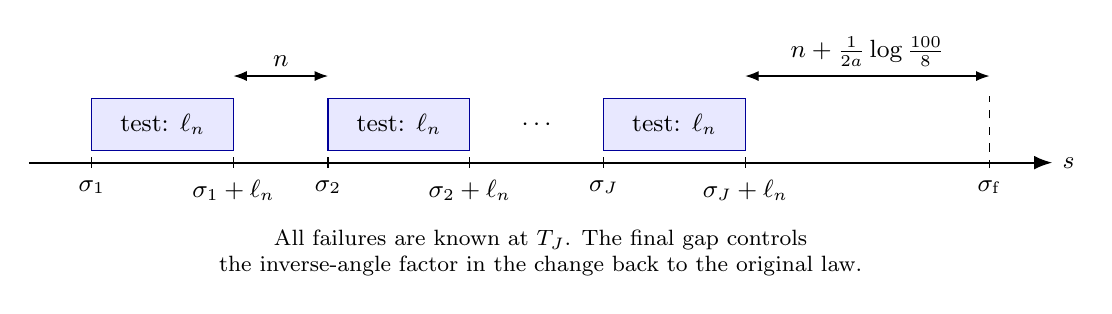
\begin{tikzpicture}[x=1cm,y=1cm,>=Latex,font=\small]
  \draw[->,thick] (0,0)--(13,0) node[right] {\(s\)};
  \foreach \x/\y in {0.8/2.6,3.8/5.6,7.3/9.1} {
    \fill[blue!9] (\x,0.15) rectangle (\y,0.82);
    \draw[blue!60!black] (\x,0.15) rectangle (\y,0.82);
    \node at ({(\x+\y)/2},0.49) {test: \(\ell_n\)};
    \draw (\x,0.07)--(\x,-0.07);
    \draw (\y,0.07)--(\y,-0.07);
  }
  \node[below] at (0.8,-0.1) {\(\sigma_1\)};
  \node[below] at (2.6,-0.1) {\(\sigma_1+\ell_n\)};
  \node[below] at (3.8,-0.1) {\(\sigma_2\)};
  \node[below] at (5.6,-0.1) {\(\sigma_2+\ell_n\)};
  \node[below] at (7.3,-0.1) {\(\sigma_J\)};
  \node[below] at (9.1,-0.1) {\(\sigma_J+\ell_n\)};
  \node at (6.45,0.48) {\(\cdots\)};
  \draw[<->] (2.6,1.1)--(3.8,1.1)
    node[midway,above] {\(n\)};
  \draw[<->] (9.1,1.1)--(12.2,1.1)
    node[midway,above] {\(n+\frac{1}{2a}\log\frac{100}{8}\)};
  \draw[dashed] (12.2,-0.07)--(12.2,0.85);
  \node[below] at (12.2,-0.1) {\(\sigma_{\mathrm f}\)};
  \node[align=center,font=\footnotesize] at (6.5,-1.15)
    {All failures are known at \(T_J\). The final gap controls\\
     the inverse-angle factor in the change back to the original law.};
\end{tikzpicture}
\caption{One batch at a fixed grid center, in inner time (schematic).
There are \(J=I_n-1\) mass tests, each of length \(\ell_n\),
with gaps \(n\) between consecutive tests. The coordinates are
\(s_z(S_i)=\sigma_i\), \(s_z(T_i)=\sigma_i+\ell_n\), and
\(s_z(\tau_{\mathrm f})=\sigma_{\mathrm f}\); the final coordinate
corresponds to conformal radius \(8r_{n,I_n}\).
The first restart is preceded by a mixing gap as well.
The tests are conditioned on their actual past; independence is unnecessary.}
\label{fig:batch-timeline}
\end{figure}

For the failure estimate, we now work under the finite centered law
stopped at \(\tau_{\mathrm f}\), under which all these levels are reached.
For all sufficiently large \(n\), each of these gaps permits
the uniform mixing estimate. Conditional on the entire stopped
history through \(T_{i-1}\), the angle at \(S_i\) has density at
least \(1/2\) relative to \(\pi_a\); the first test has the same
bound from its initial gap.
Conditional on the history through \(S_i\), the disk law of
\(X_i\) depends only on that angle, by
Proposition~\ref{mass:restart} and the finite conditional tilt.
Thus, with
\[
 q_i=\PP^*_{\mathrm{mix}}(L_{\ell_n}\ge b_i),
\]
the conditional probability of success is at least \(q_i/2\).
Iterated conditional expectations, followed by
Lemma~\ref{gauge:multiplicity}, give
\begin{equation}
 \PP_z^*(X_i<b_i\text{ for every }i\le J)
 \le\prod_{i=1}^J(1-q_i/2)
 \le \exp\left(-\tfrac12\sum_{i=1}^Jq_i\right)
 \le \exp(-2^n/16).
 \label{hd:test-failure}
\end{equation}
This argument conditions on the actual past at each test.
It requires no independence between tests or between centers.

\paragraph{Changing law for the failure event.}
The event that a cell is visited and has no candidate is
contained in the larger event
\begin{equation}
 A=\{\tau_{\mathrm f}<\infty\}
       \cap\bigcap_{i=1}^J\{X_i<b_i\}.
 \label{hd:adapted-enlargement}
\end{equation}
All test endpoints precede \(\tau_{\mathrm f}\), so \(A\) is
measurable at that stopping time. Only this enlarged event is
used in changing law. In particular, no terminal candidate
information is put into a finite Radon--Nikodym formula.
Let \(\widehat\theta=\theta_{\tau_{\mathrm f}}(z)\) and
\(F_{\mathrm{fail}}=\bigcap_i\{X_i<b_i\}\).
The final gap in Equation~\eqref{hd:test-gaps}, conditional on
the history through \(T_J\), gives
\[
 \EE_z^*[\sin^{-p}\widehat\theta\mid\mathcal F_{T_J}]
 \le 2\int\sin^{-p}\theta\,\pi_a(\dd\theta).
\]
Since \(F_{\mathrm{fail}}\) is known at \(T_J\), the density at
\(\tau_{\mathrm f}\) and Equation~\eqref{hd:test-failure} yield
\begin{align}
 &\PP(\text{the cell at }z\text{ is visited and has no candidate})
 \notag\\
 &\quad\le\PP(A)
  =(8r_{\mathrm f})^\alpha G_0(z)\,
       \EE_z^*[\sin^{-p}\widehat\theta;\ F_{\mathrm{fail}}]
 \notag\\
 &\quad\le C_a r_{\mathrm f}^{\alpha}y^{-\alpha}
                       \exp(-2^n/16)
       \qquad(y\ge e^{-n}).
 \label{hd:upper-cell}
\end{align}
For centers below \(e^{-n}\), use the unconditional estimate
\begin{equation}
 \PP(\text{the cell at }z\text{ is visited})
 \le C_a r_{\mathrm f}^{\alpha}y^{-\alpha}
 \label{hd:lower-cell}
\end{equation}
from Lemma~\ref{hd:visit}. This includes the bottom row:
its center has height \(r_{\mathrm f}/2\), and the trivial
probability bound is absorbed by the displayed estimate.

\paragraph{Selecting and charging the cover.}
Order all candidate balls by
decreasing radius, using a fixed deterministic order for ties.
Choose the first ball, delete every ball meeting it, and
continue until no candidates remain. The selected closed balls
are pairwise disjoint. A deleted ball has radius no greater
than that of the ball that deletes it, so it is contained in
the concentric triple of that selected ball.
The triples therefore cover every final cell having a candidate.
For a chosen ball associated with \((b_i,r_i)\), its triple
has diameter \(6C_*r_i\); Equation~\eqref{gauge:definition}
and its qualification give
\begin{align}
 h(6C_*r_i)
 &\le (6C_*)^2 b_i r_i^d \notag\\
 &\le \frac{(6C_*)^2}{c_*^d}\,
       \mu_\infty\bigl(\overline B(z,C_*r_i)\cap\HH\bigr).
 \label{hd:candidate-cost}
\end{align}
For large \(n\) all these balls lie, after intersection with
\(\HH\), in the fixed bounded set
\[
 \widetilde B_m=[-m-2,m+2]+i(0,m+2].
\]
Disjointness thus bounds their total gauge cost by
\[
 \frac{(6C_*)^2}{c_*^d}\,\mu_\infty(\widetilde B_m).
\]
This is the actual mass of a fixed region on the same sample.
It has finite expectation, even at the real boundary:
\begin{equation}
 \EE\mu_\infty(\widetilde B_m)
 =\int_{\widetilde B_m}G_0(z)\,\dd A(z)
 \le \frac{2^{-\alpha}(2m+4)(m+2)^{1-\alpha}}{1-\alpha}
 <\infty.
 \label{hd:boundary-integrability}
\end{equation}
The mean identity on this set follows by an interior compact
exhaustion and monotone convergence.

\paragraph{Paying for missed cells and the boundary.}
Add every final cell that meets $\Gamma$ and has no candidate.
The cleanup entry gives the individual cost
\[
 h(\sqrt2\,r_{\mathrm f})\le2n r_{\mathrm f}^d.
\]
There are \(O_m(r_{\mathrm f}^{-1})\) columns. Since
\(0<\alpha<1\), summing the half-integer row heights gives
\begin{align*}
 \sum_{\text{all cells}}y^{-\alpha}
     &\le C_{a,m}r_{\mathrm f}^{-2},\\
 \sum_{y<e^{-n}}y^{-\alpha}
     &\le C_{a,m}r_{\mathrm f}^{-2}
                        (e^{-n}+r_{\mathrm f})^{1-\alpha}.
\end{align*}
For example,
\(\sum_{j=0}^N(j+\tfrac12)^{-\alpha}
\le C_\alpha(N+1)^{1-\alpha}\) proves both bounds.
Multiplying Equations~\eqref{hd:upper-cell} and
\eqref{hd:lower-cell} by the cleanup cost, and using
\(d+\alpha=2\), bounds the expected added cost by
\begin{equation}
 C_{a,m}\left[
       n e^{-2^n/16}
       +n(e^{-n}+r_{\mathrm f})^{1-\alpha}
       \right].
 \label{hd:cleanup-cost}
\end{equation}
It is bounded uniformly in \(n\) and tends to zero.
In particular, the bottom row contributes at most
\(C_m n r_{\mathrm f}^{d-1}\). Thus points of the trace on
the real axis are included in the cover, although the auxiliary
mass itself is defined on \(\HH\).

\paragraph{Measurability and the limiting cover.}
These constructions are measurable. The candidate family is
finite with measurable terminal-mass indicators, and the
greedy order is deterministic. For a fixed closed cell, the
event of meeting the trace is measurable on every compact time
interval, by continuity; a countable union over integer time
horizons gives the full trace event.
All upper-bound centers, entries, and boxes constitute a
countable family, so the stopped measure identities used in
constructing their tests can be imposed on one event.

Let \(C_n\) be the total gauge cost of the resulting cover of
\(\Gamma\cap B_m\). Equations~\eqref{hd:candidate-cost}--%
\eqref{hd:cleanup-cost} show that
\(\sup_n\EE C_n<\infty\), after omitting finitely many initial
batches. Every cover diameter is at most
\[
 \delta_n=6C_*e^{-n^2},
\]
which tends deterministically to zero.
Fatou's Lemma gives
\[
 \EE[\liminf_{n\to\infty}C_n]
 \le\liminf_{n\to\infty}\EE C_n<\infty,
\]
so the liminf cost is finite almost surely.
For every fixed \(\delta>0\), all sufficiently late covers are
admissible for \(\Haus^h_\delta(\Gamma\cap B_m)\), and hence
\[
 \Haus^h_\delta(\Gamma\cap B_m)
 \le\liminf_{n\to\infty}C_n.
\]
Letting $\delta\downarrow0$ gives the pathwise domination
\begin{equation}
 \Haus^h(\Gamma\cap B_m)\le\liminf_{n\to\infty}C_n.
 \label{hd:liminf-domination}
\end{equation}

We justify ordinary expectation of the left side. For an integer $T$,
$K_T=\gamma([0,T])\cap B_m$ is a measurable compact random set.
Indeed, for a fixed closed $F$, the event $K_T\cap F\ne\varnothing$
is the measurable event
$\min_{0\le t\le T}\dist(\gamma(t),B_m\cap F)=0$; the minimum can
be computed on rational times. Empty target sets give the empty event.
Hit events for open sets follow by an increasing union of closed
subsets, so these tests give the required compact-set measurability.
Intersection with $B_m$ need not depend continuously on the path.

For completeness, $K\mapsto\Haus^h(K)$ is measurable on compact sets.
Use the countable family of finite unions of open balls with rational
centers and radii. The limit of the corresponding countable infima
over finite covers, with their diameter cutoff tending to zero, equals
$\Haus^h(K)$. To see this, start with any countable cover of the compact
$K$ at a smaller cutoff. Enlarge its sets to open neighborhoods with
arbitrarily small diameter slack and summable cost slack, using
continuity of $h$ (also at zero). Compactness gives a finite subcover.
Shrink that finite cover on $K$ to compact pieces, and cover each piece
by finitely many rational balls inside its assigned neighborhood.
The grouped balls remain inside that neighborhood, preserving its
diameter bound and cost. This proves equality after letting the cutoff
and slack tend to zero; equality at an unchanged fixed cutoff is not
needed. Each admissibility event $K\subset O$ for a fixed open $O$
is measurable, so the countable infima and their limit are measurable.

Finally $\Gamma\cap B_m=\bigcup_{T\in\mathbb N}K_T$ is an increasing
union of compact sets. Hausdorff outer measure is a measure on Borel
sets, so continuity from below gives
$\Haus^h(\Gamma\cap B_m)=\lim_T\Haus^h(K_T)$.
This is measurable. Taking expectations in
\eqref{hd:liminf-domination} and applying the preceding Fatou bound
proves \eqref{hd:expected-box}. A countable intersection now gives
almost-sure finiteness in every integer box.
\end{proof}

\begin{proof}[Proof of Theorem~\ref{thm:main}]
Equation~\eqref{coef:formula} specifies the coefficients
deterministically from \(\kappa\), and
Proposition~\ref{gauge:admissible} shows that
Equation~\eqref{gauge:definition} defines an admissible gauge.
Intersect the probability-one events of
Propositions~\ref{hd:lower} and~\ref{hd:upper}.
On this one event, the lower bound holds for every real
\(0<s<t<\infty\).
The image of each finite time interval is bounded by continuity
of \(\gamma\), and therefore lies in one of the integer boxes
of Proposition~\ref{hd:upper}; its Hausdorff measure is finite.
Thus the required positive finite measure holds simultaneously
for every such interval. The constant change of capacity time
used at the start preserves this all-interval assertion.
\end{proof}

\bibliographystyle{plain}
\bibliography{refs/sources}
\end{document}
